\documentclass{article}
\title{Intro to PDEs: Ch 5.1-5.2 HW}
\author{Logan Rhyne, Harley Combest, Roy Galang, Jesse DiCenso}
\usepackage[T1]{fontenc}
\usepackage{amsfonts, amsmath, amsthm, amssymb}
\usepackage{mathtools, bigints, empheq}
\usepackage{graphicx, wrapfig, xcolor, float}
\usepackage{stackrel}
\usepackage{pgfplots}
\usepackage[shortlabels]{enumitem}
\usepackage[margin=1.0in]{geometry}
\setlength{\parindent}{0pt}
\theoremstyle{definition}
\newtheorem*{lemma}{Lemma}
\newtheorem*{conj}{Conjecture}
\newtheorem{prob}{}
\newtheorem*{pf}{Proof}
\newtheorem*{dpf}{Disproof}
\renewcommand\qedsymbol{$\blacksquare$}
\renewcommand{\emptyset}{\varnothing}
\renewcommand{\epsilon}{\varepsilon}
\newenvironment{disproof}{\begin{proof}[Disproof]}{\end{proof}}
\newenvironment{ans}{\begin{proof}[Answer]\renewcommand{\qedsymbol}{}}{\end{proof}}
\newenvironment{boldenv}{\bfseries\boldmath}{}
\newcommand{\N}{\mathbb{N}}
\newcommand{\Z}{\mathbb{Z}}
\newcommand{\R}{\mathbb{R}}

\pgfplotsset{compat=1.18}

\DeclareMathOperator{\ran}{range}

\begin{document}

\maketitle

For this homework assignment, we will use the Fourier transform formula:
\begin{figure}[H]
    \centering
    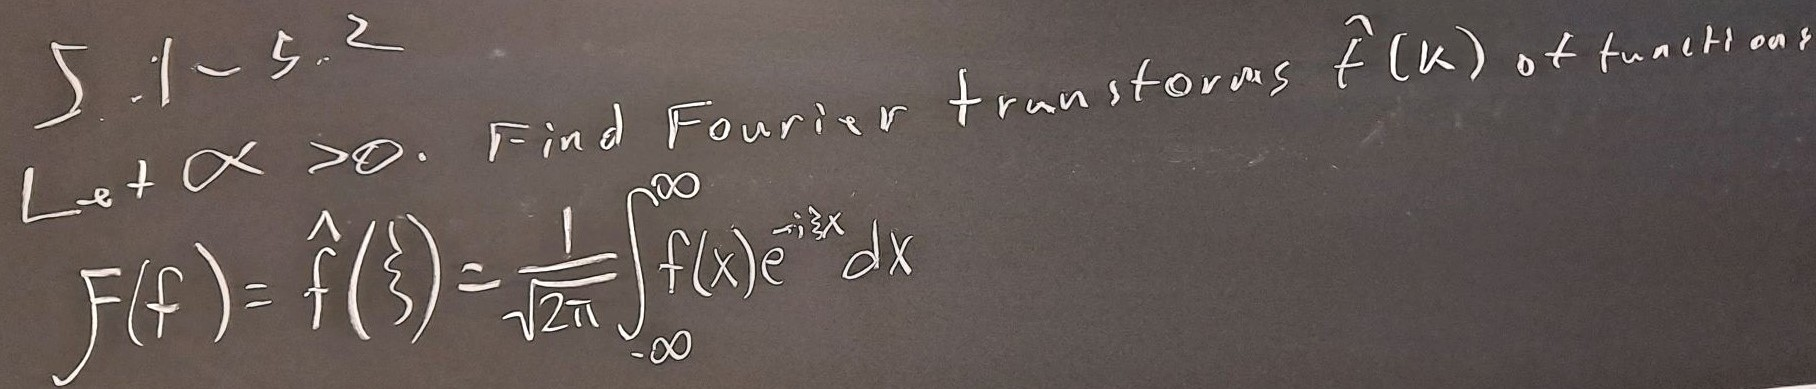
\includegraphics[width = 0.75\textwidth]{Fourier transform equation.jpeg}
\end{figure}
In addition, the problems will also utilize this property very often:
\begin{align*}
    & \text{Given} f(x) = x g(x),\\
    & \hat{f}(\xi) = i \partial_\xi{\hat{g}(\xi)}
\end{align*}

\begin{boldenv}
    \underline{Problem 2}. Let $\alpha > 0$. Find Fourier transforms $\hat{f}(k)$ of functions \begin{align}
        & f(x)=e^{-\alpha |x|}\\
        & f(x)=\begin{cases}
            e^{-\alpha x} & \mkern 50mu x > 0,\\
            0 & \mkern 50mu x \leq 0
        \end{cases}\\
        & f(x)=\begin{cases}
            x e^{-\alpha x} & \mkern 50mu x > 0,\\
            0 & \mkern 50mu x \leq 0
        \end{cases}\\
        & f(x)=e^{-\alpha |x|} \cos{\beta x}\\
        & f(x)=e^{-\alpha |x|} \sin{\beta x}\\
        & f(x)=x e^{-\alpha |x|}\\
        & f(x)=x e^{-\alpha |x|} \cos{\beta x}\\
        & f(x)=x e^{-\alpha |x|} \sin{\beta x}\\
        & f(x)=x^2 e^{-\alpha |x|}
    \end{align}
\end{boldenv}

\begin{ans}
    \begin{enumerate}
        \item \phantom{.}
        \begin{figure}[H]
            \centering
            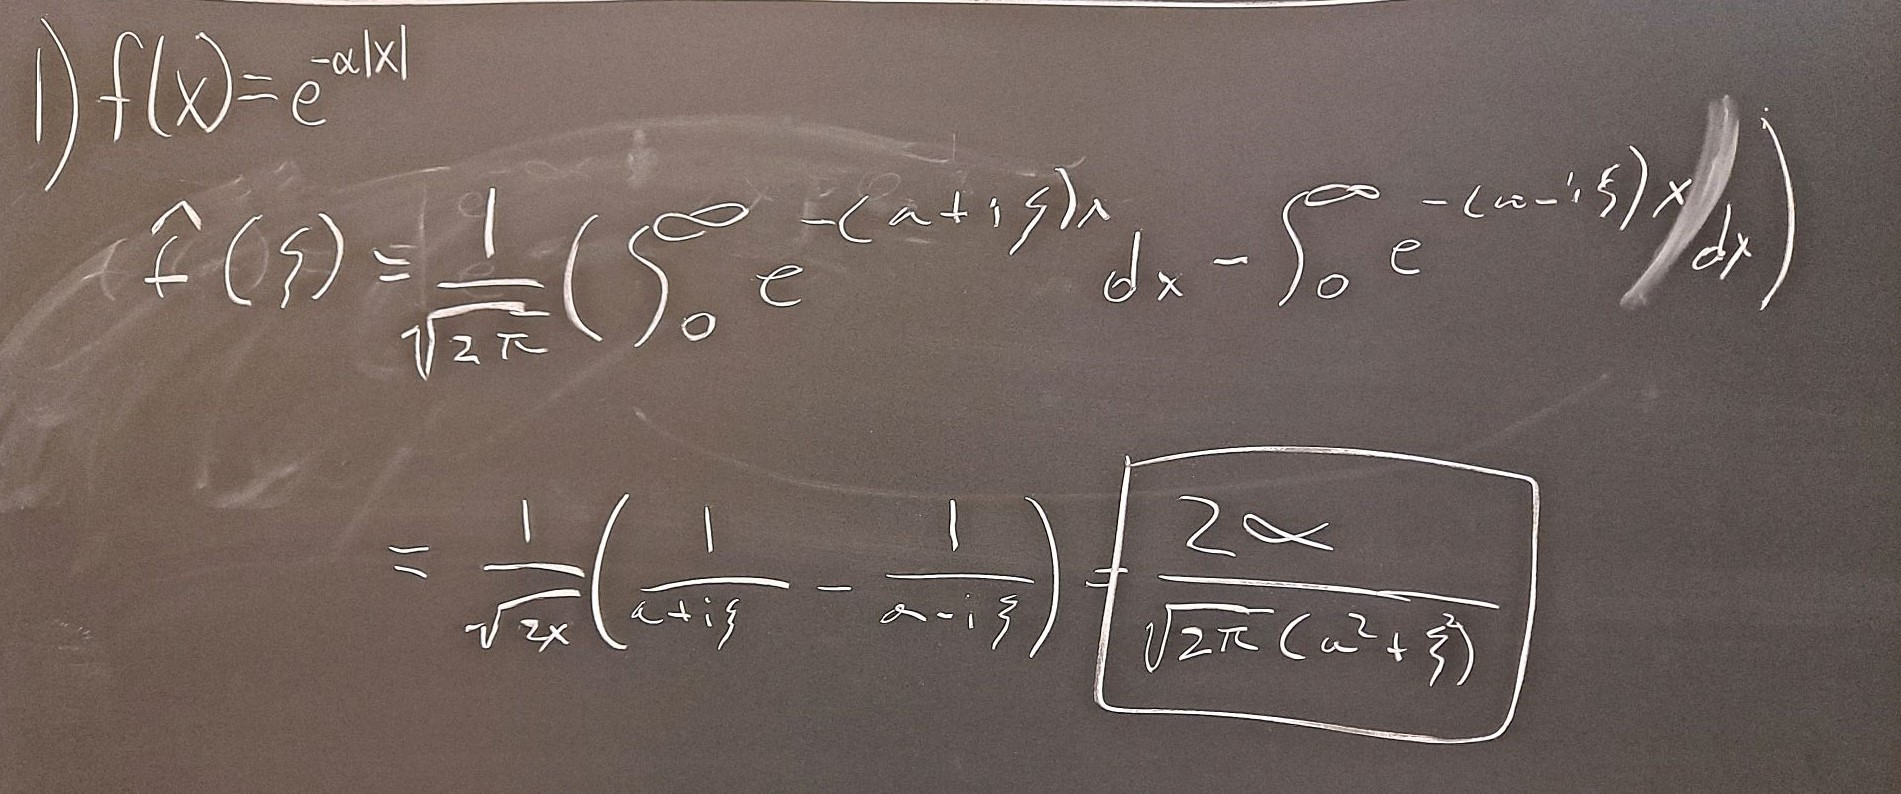
\includegraphics[width = 0.75\textwidth]{Problem 2 Part 1.jpeg}
        \end{figure}

        \item \phantom{.}
        \begin{figure}[H]
            \centering
            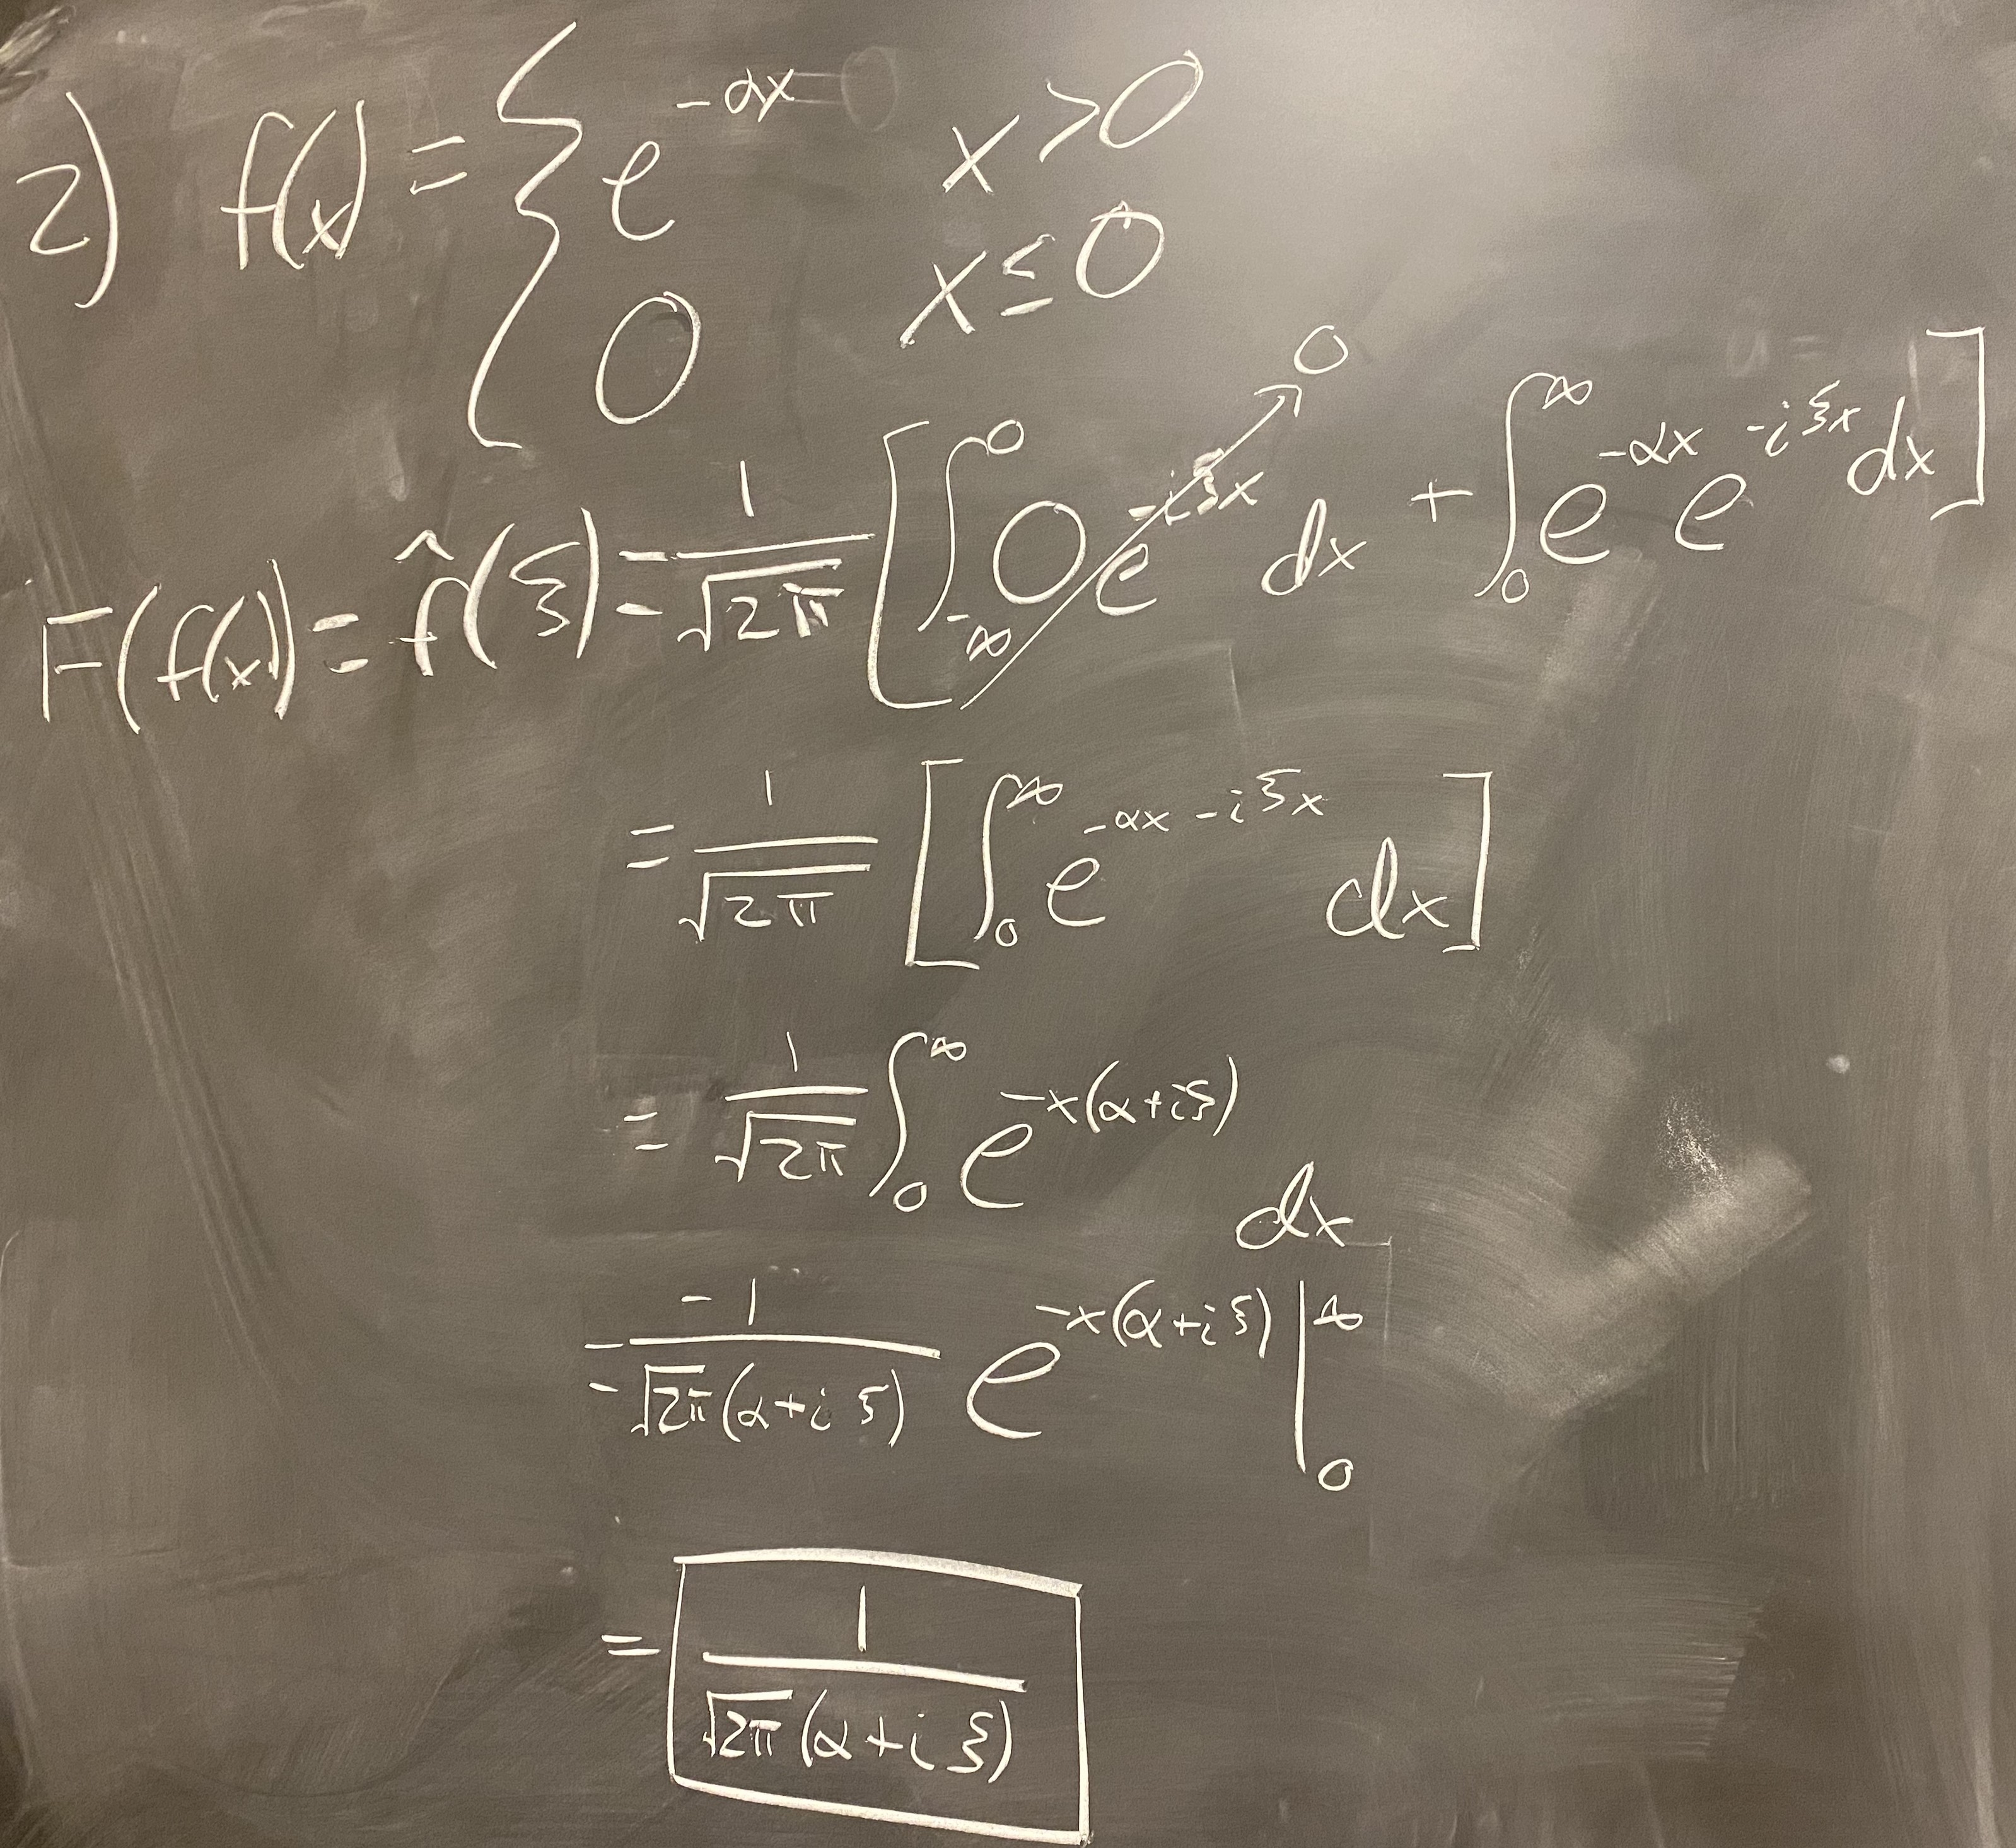
\includegraphics[width = 0.75\textwidth]{Problem 2 Part 2.jpeg}
        \end{figure}

        \item \phantom{.}
        \begin{figure}[H]
            \centering
            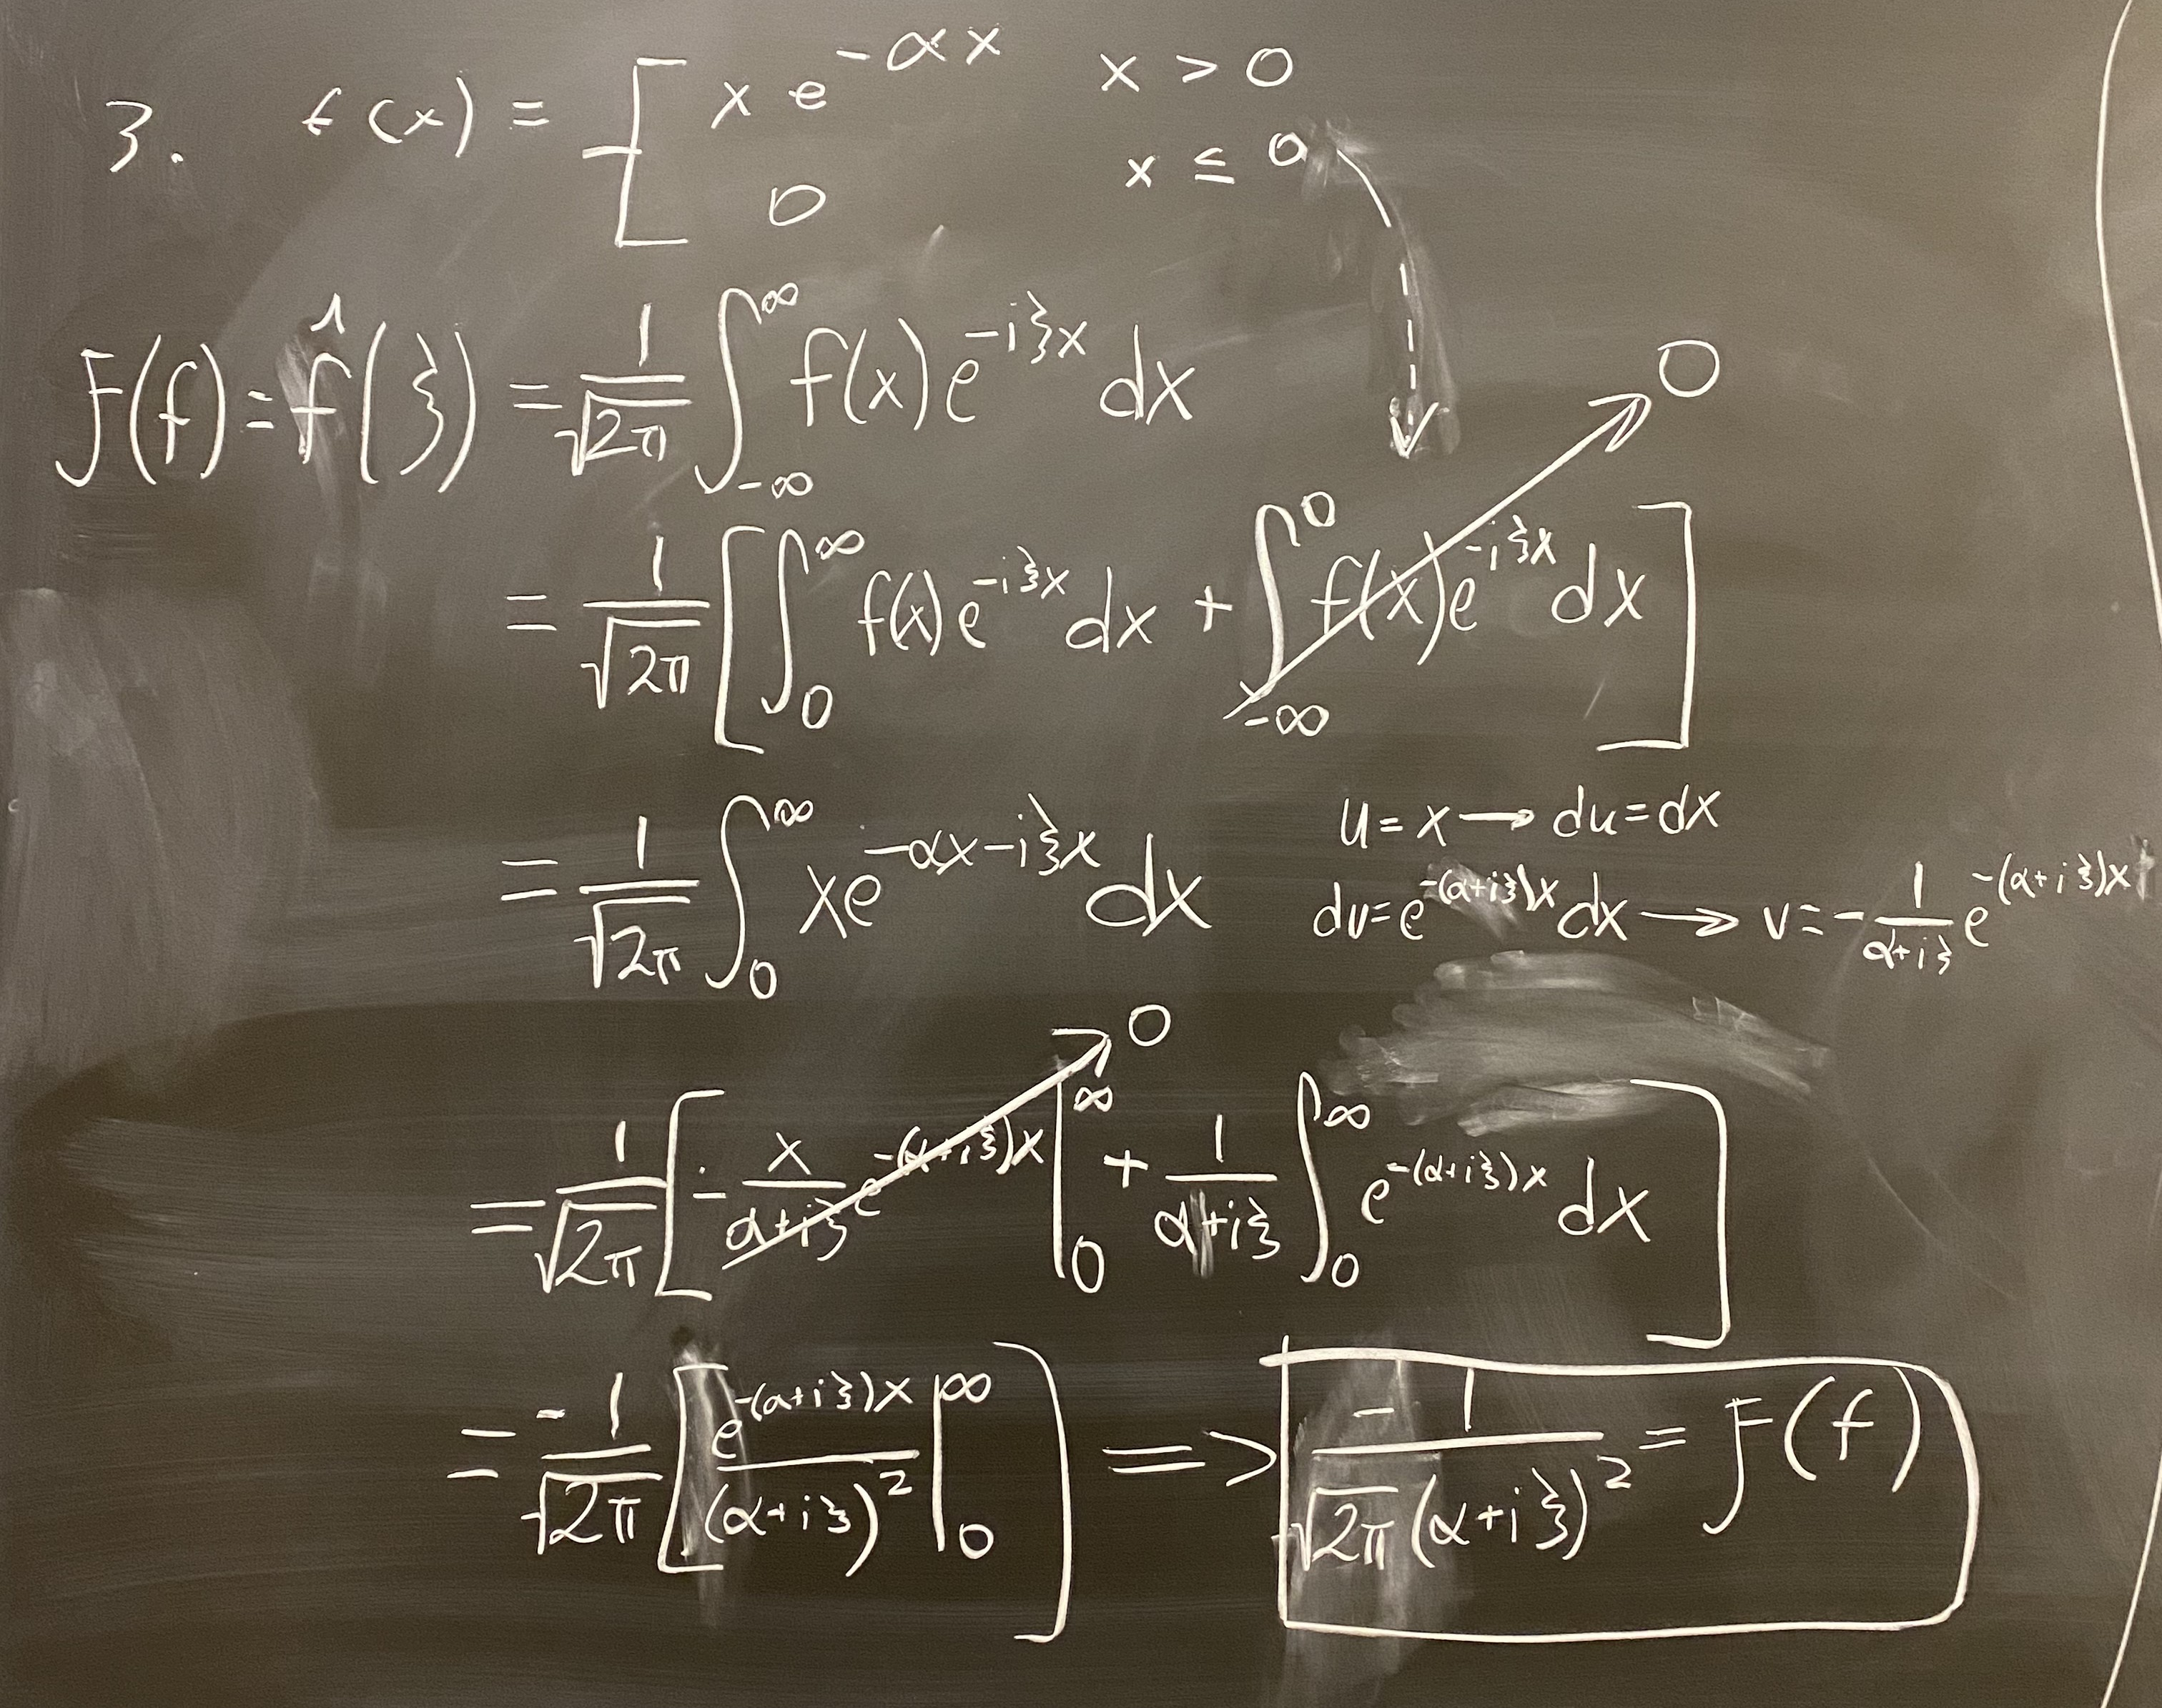
\includegraphics[width = 0.75\textwidth]{Problem 2 Part 3.jpeg}
        \end{figure}

        \item \phantom{.}
        \begin{figure}[H]
            \centering
            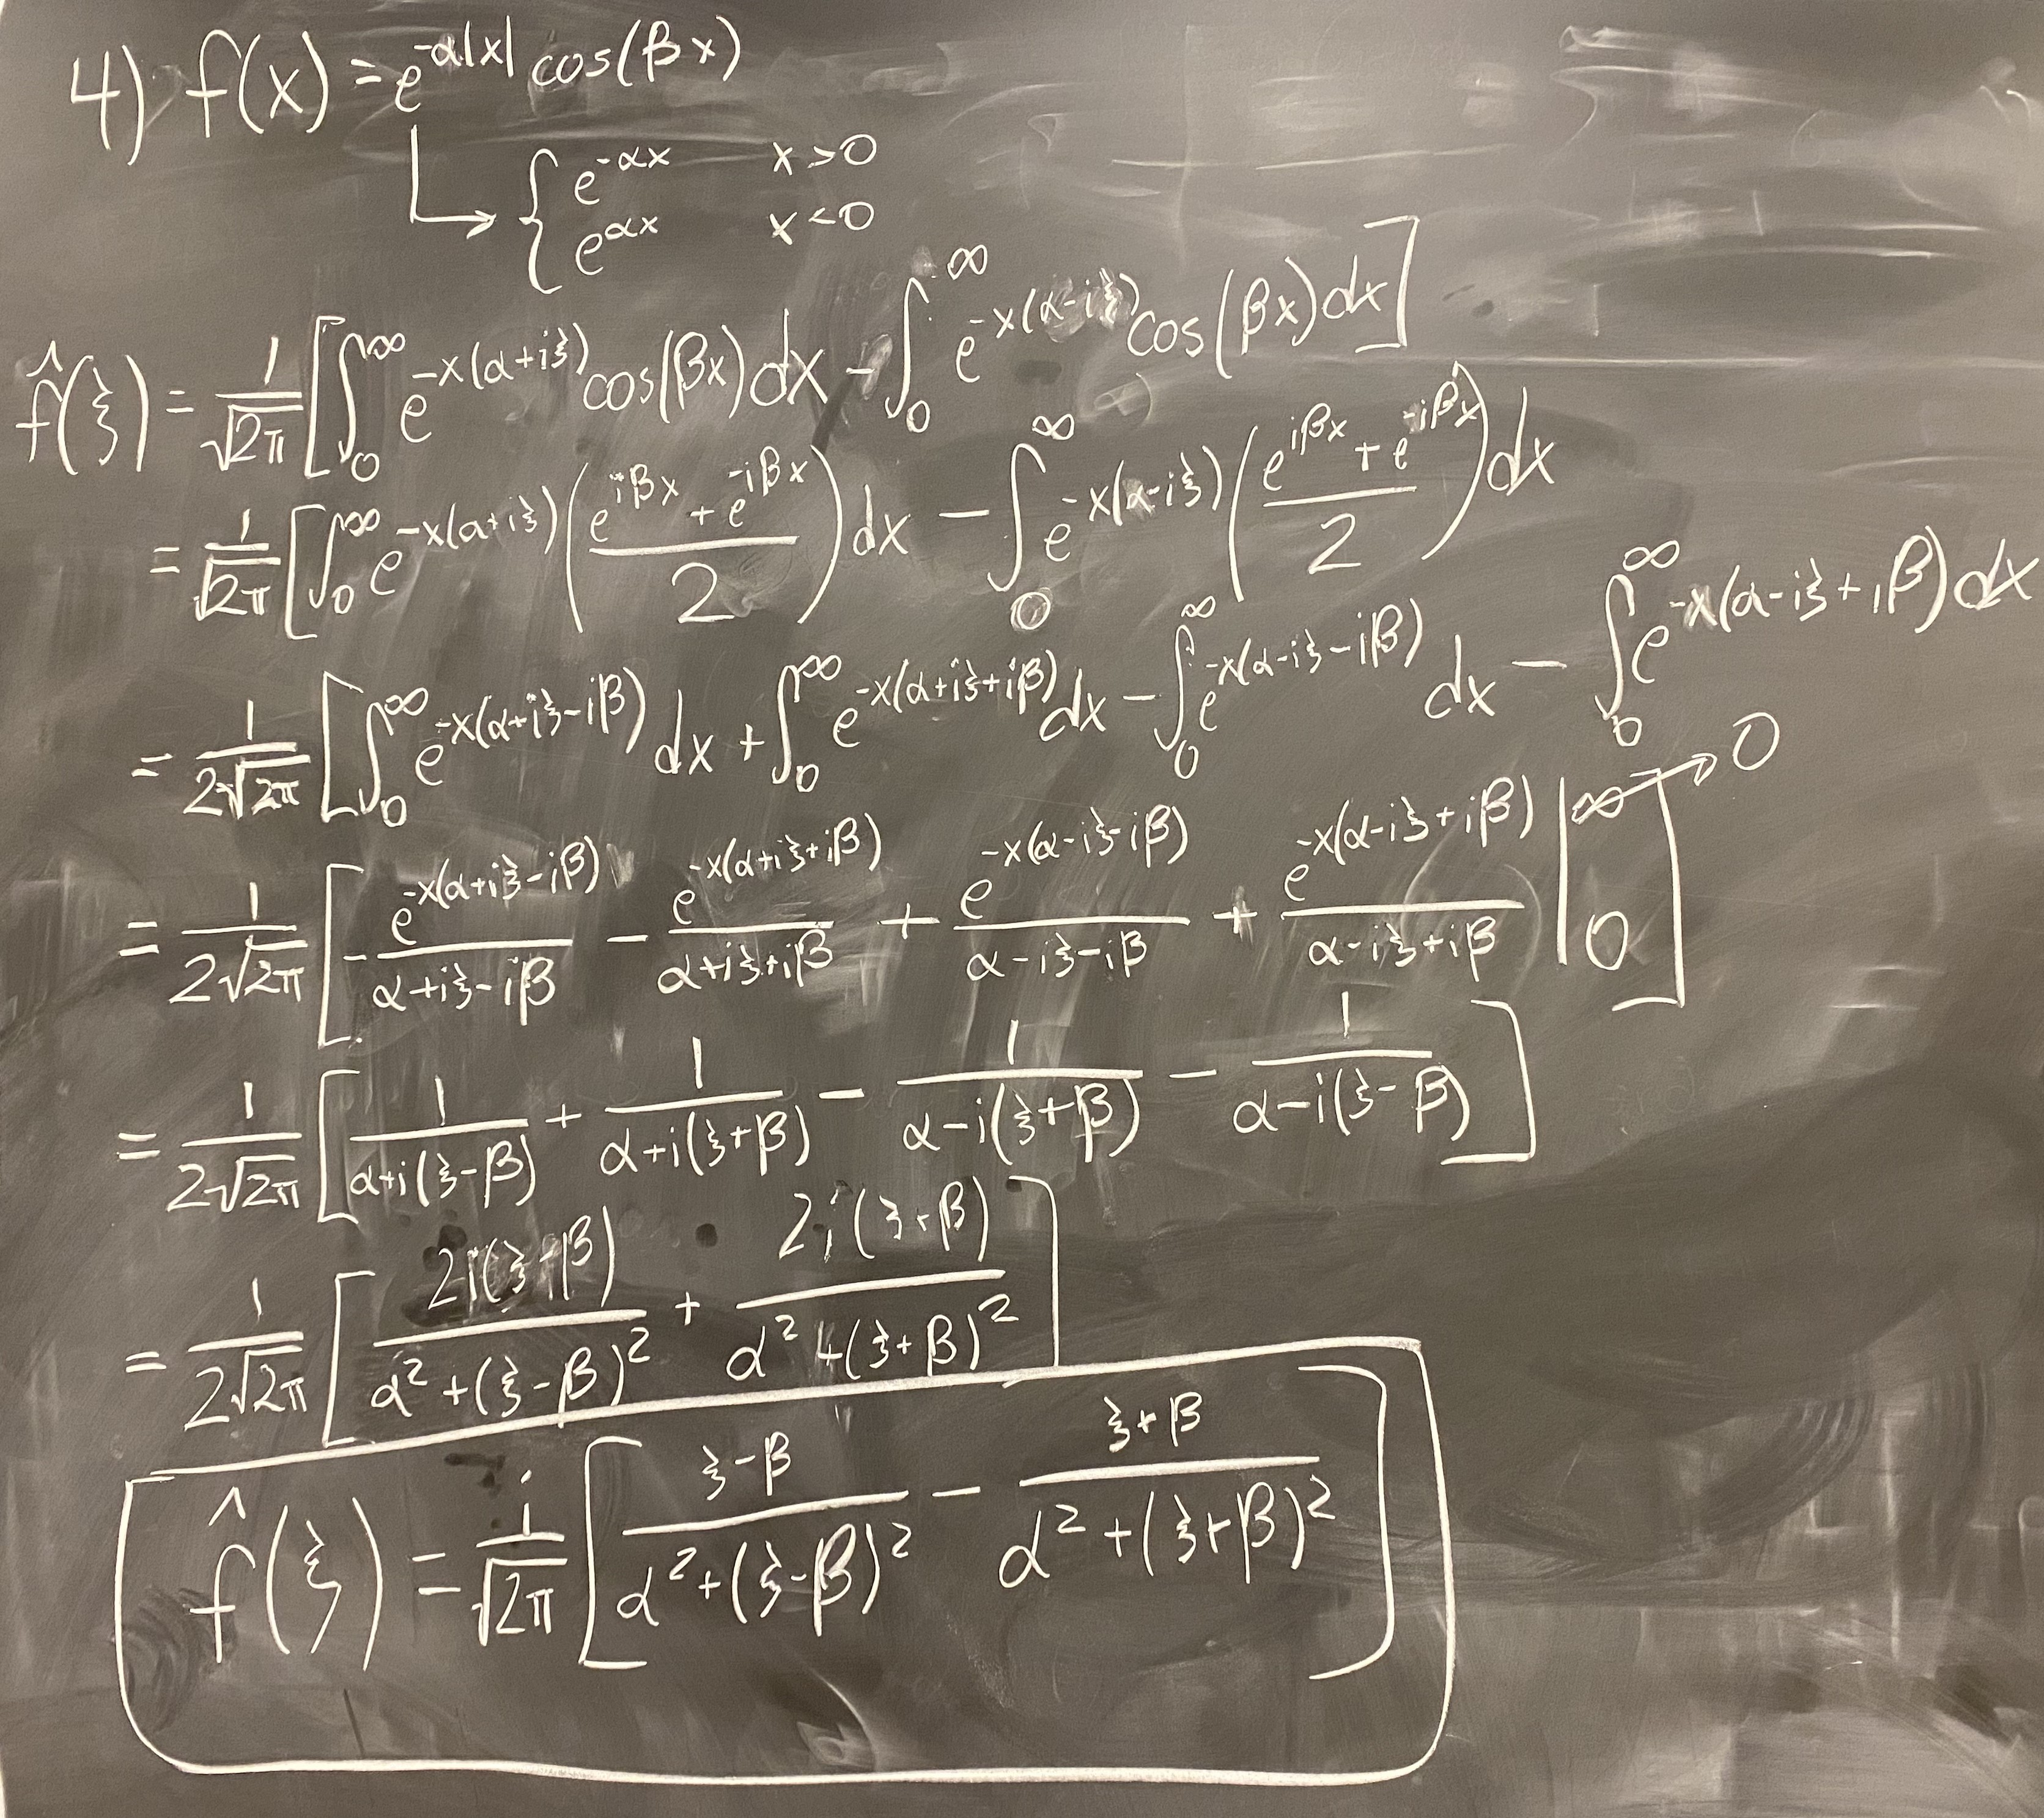
\includegraphics[width = 0.75\textwidth]{Problem 2 Part 4.jpeg}
        \end{figure}

        \item \phantom{.}
        \begin{figure}[H]
            \centering
            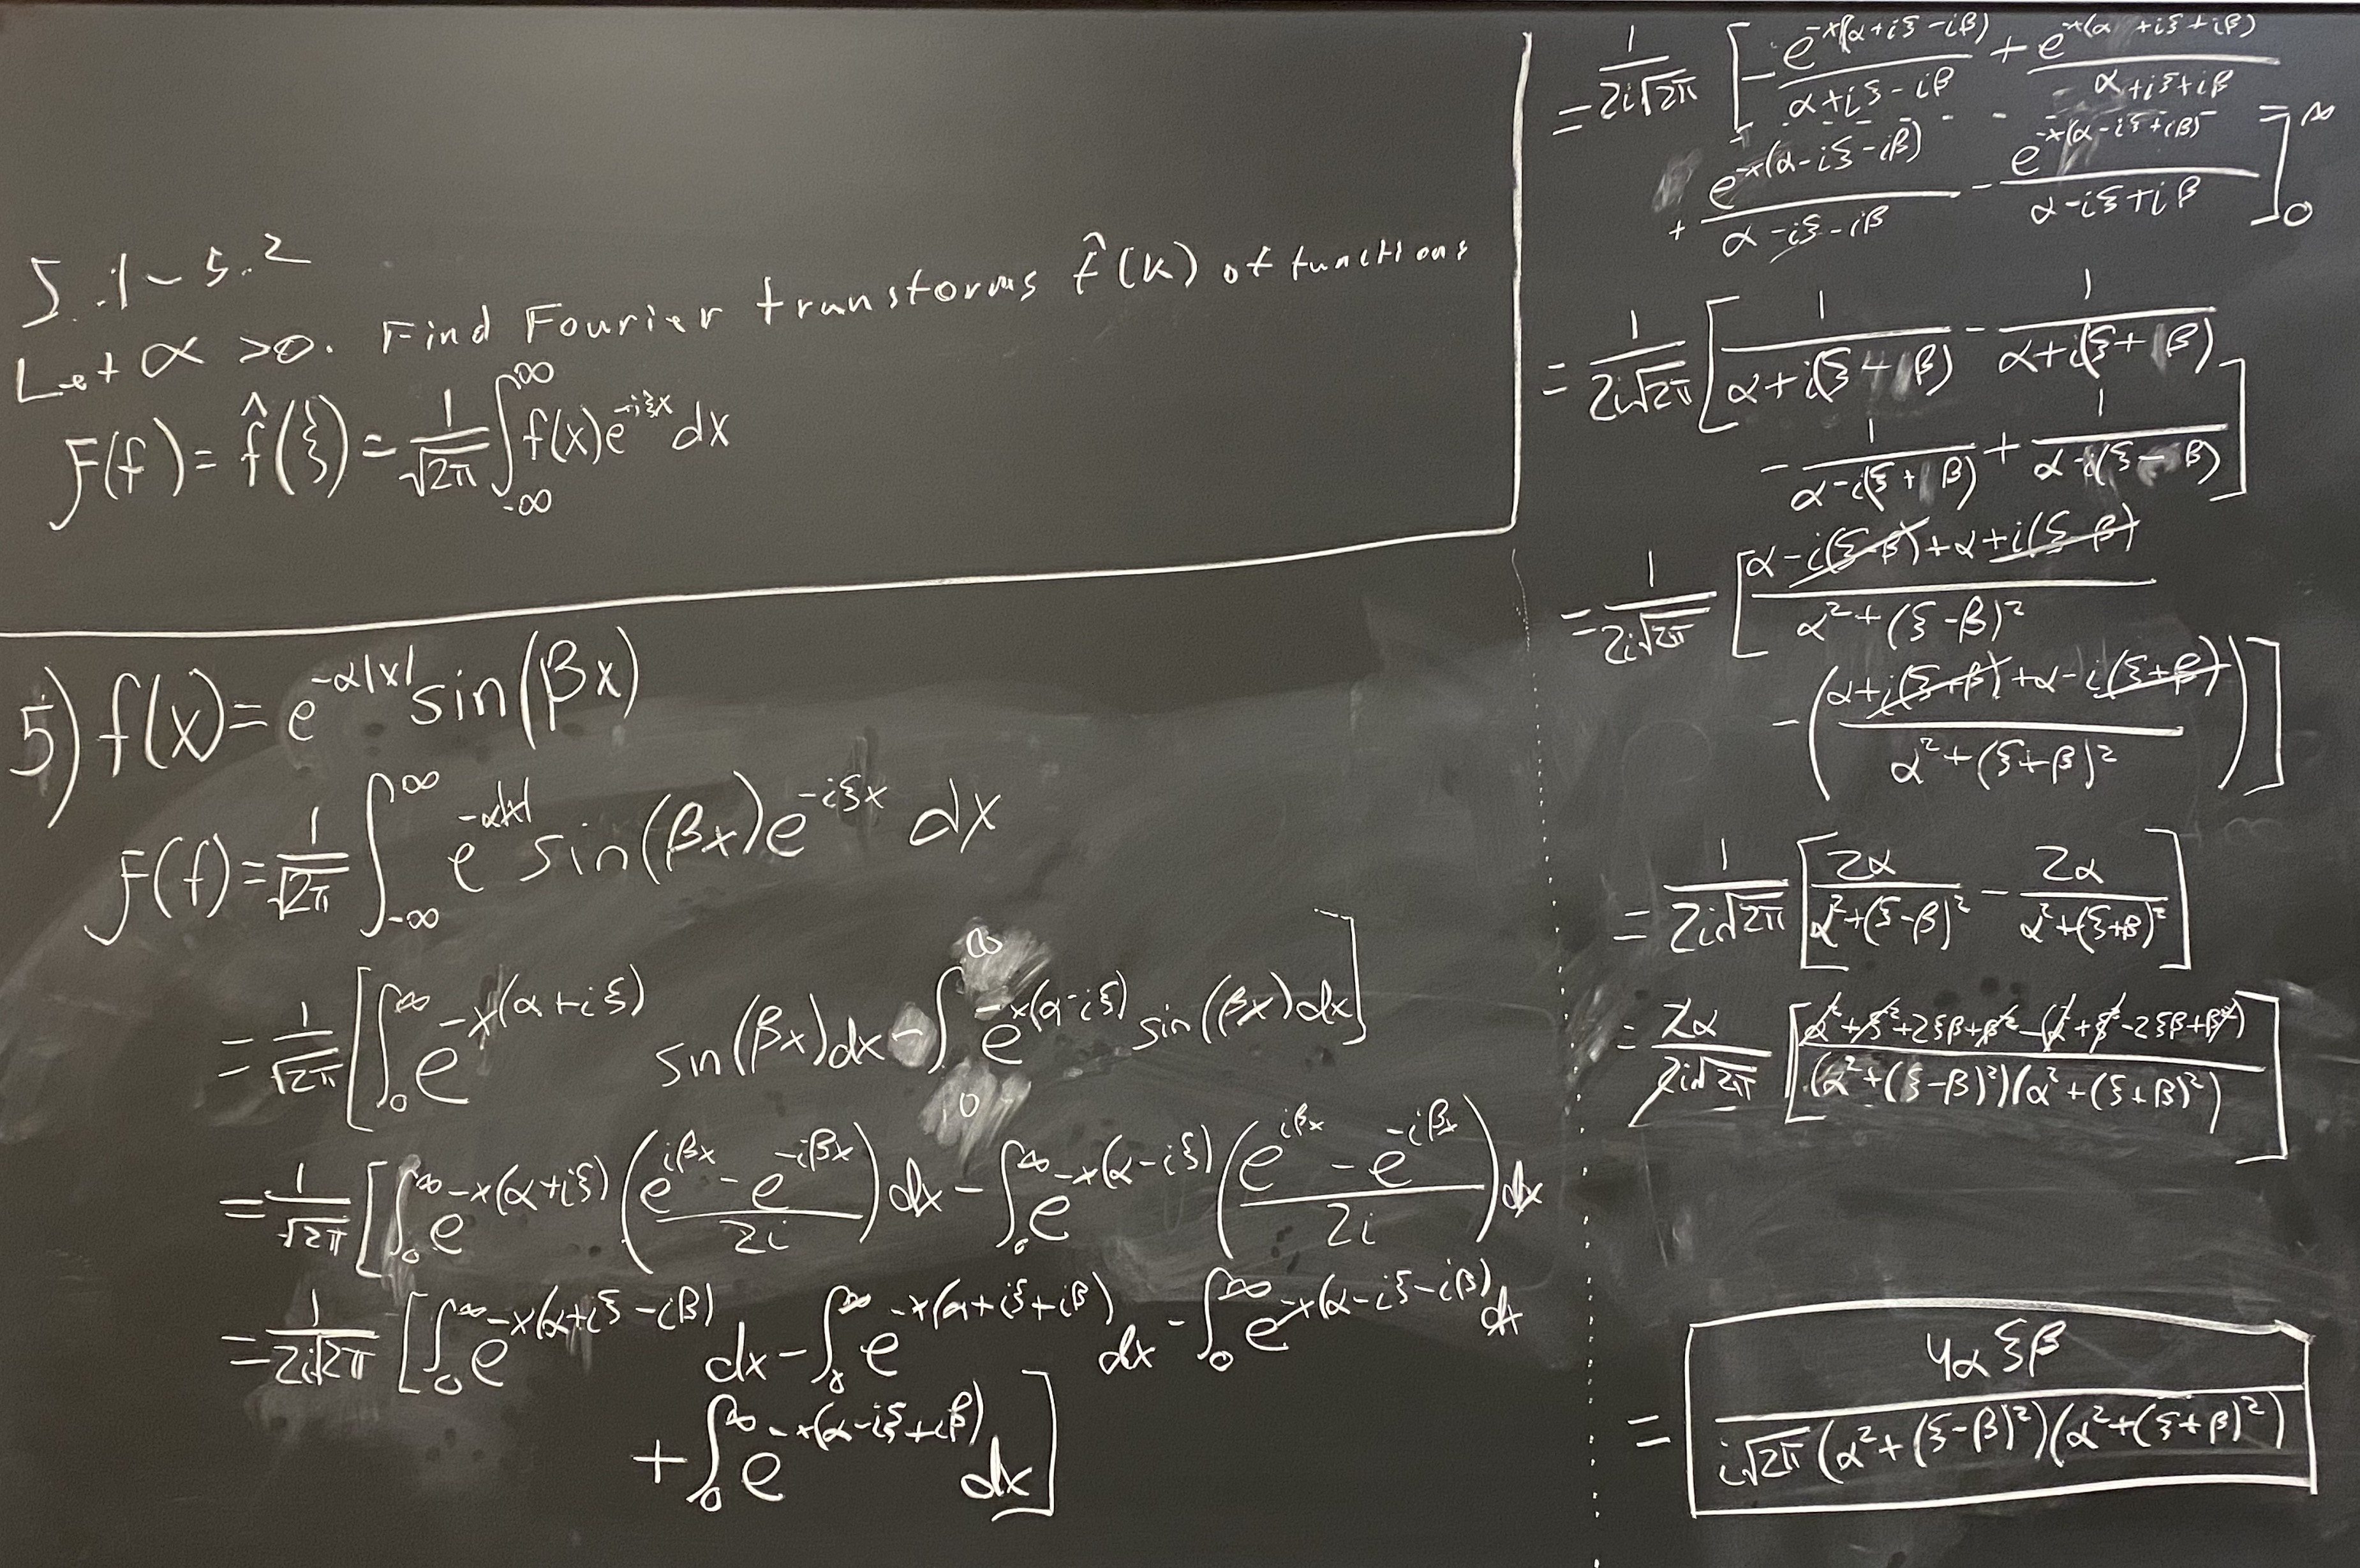
\includegraphics[width = 0.75\textwidth]{Problem 2 Part 5.jpeg}
        \end{figure}

        \item \phantom{.}
        \begin{figure}[H]
            \centering
            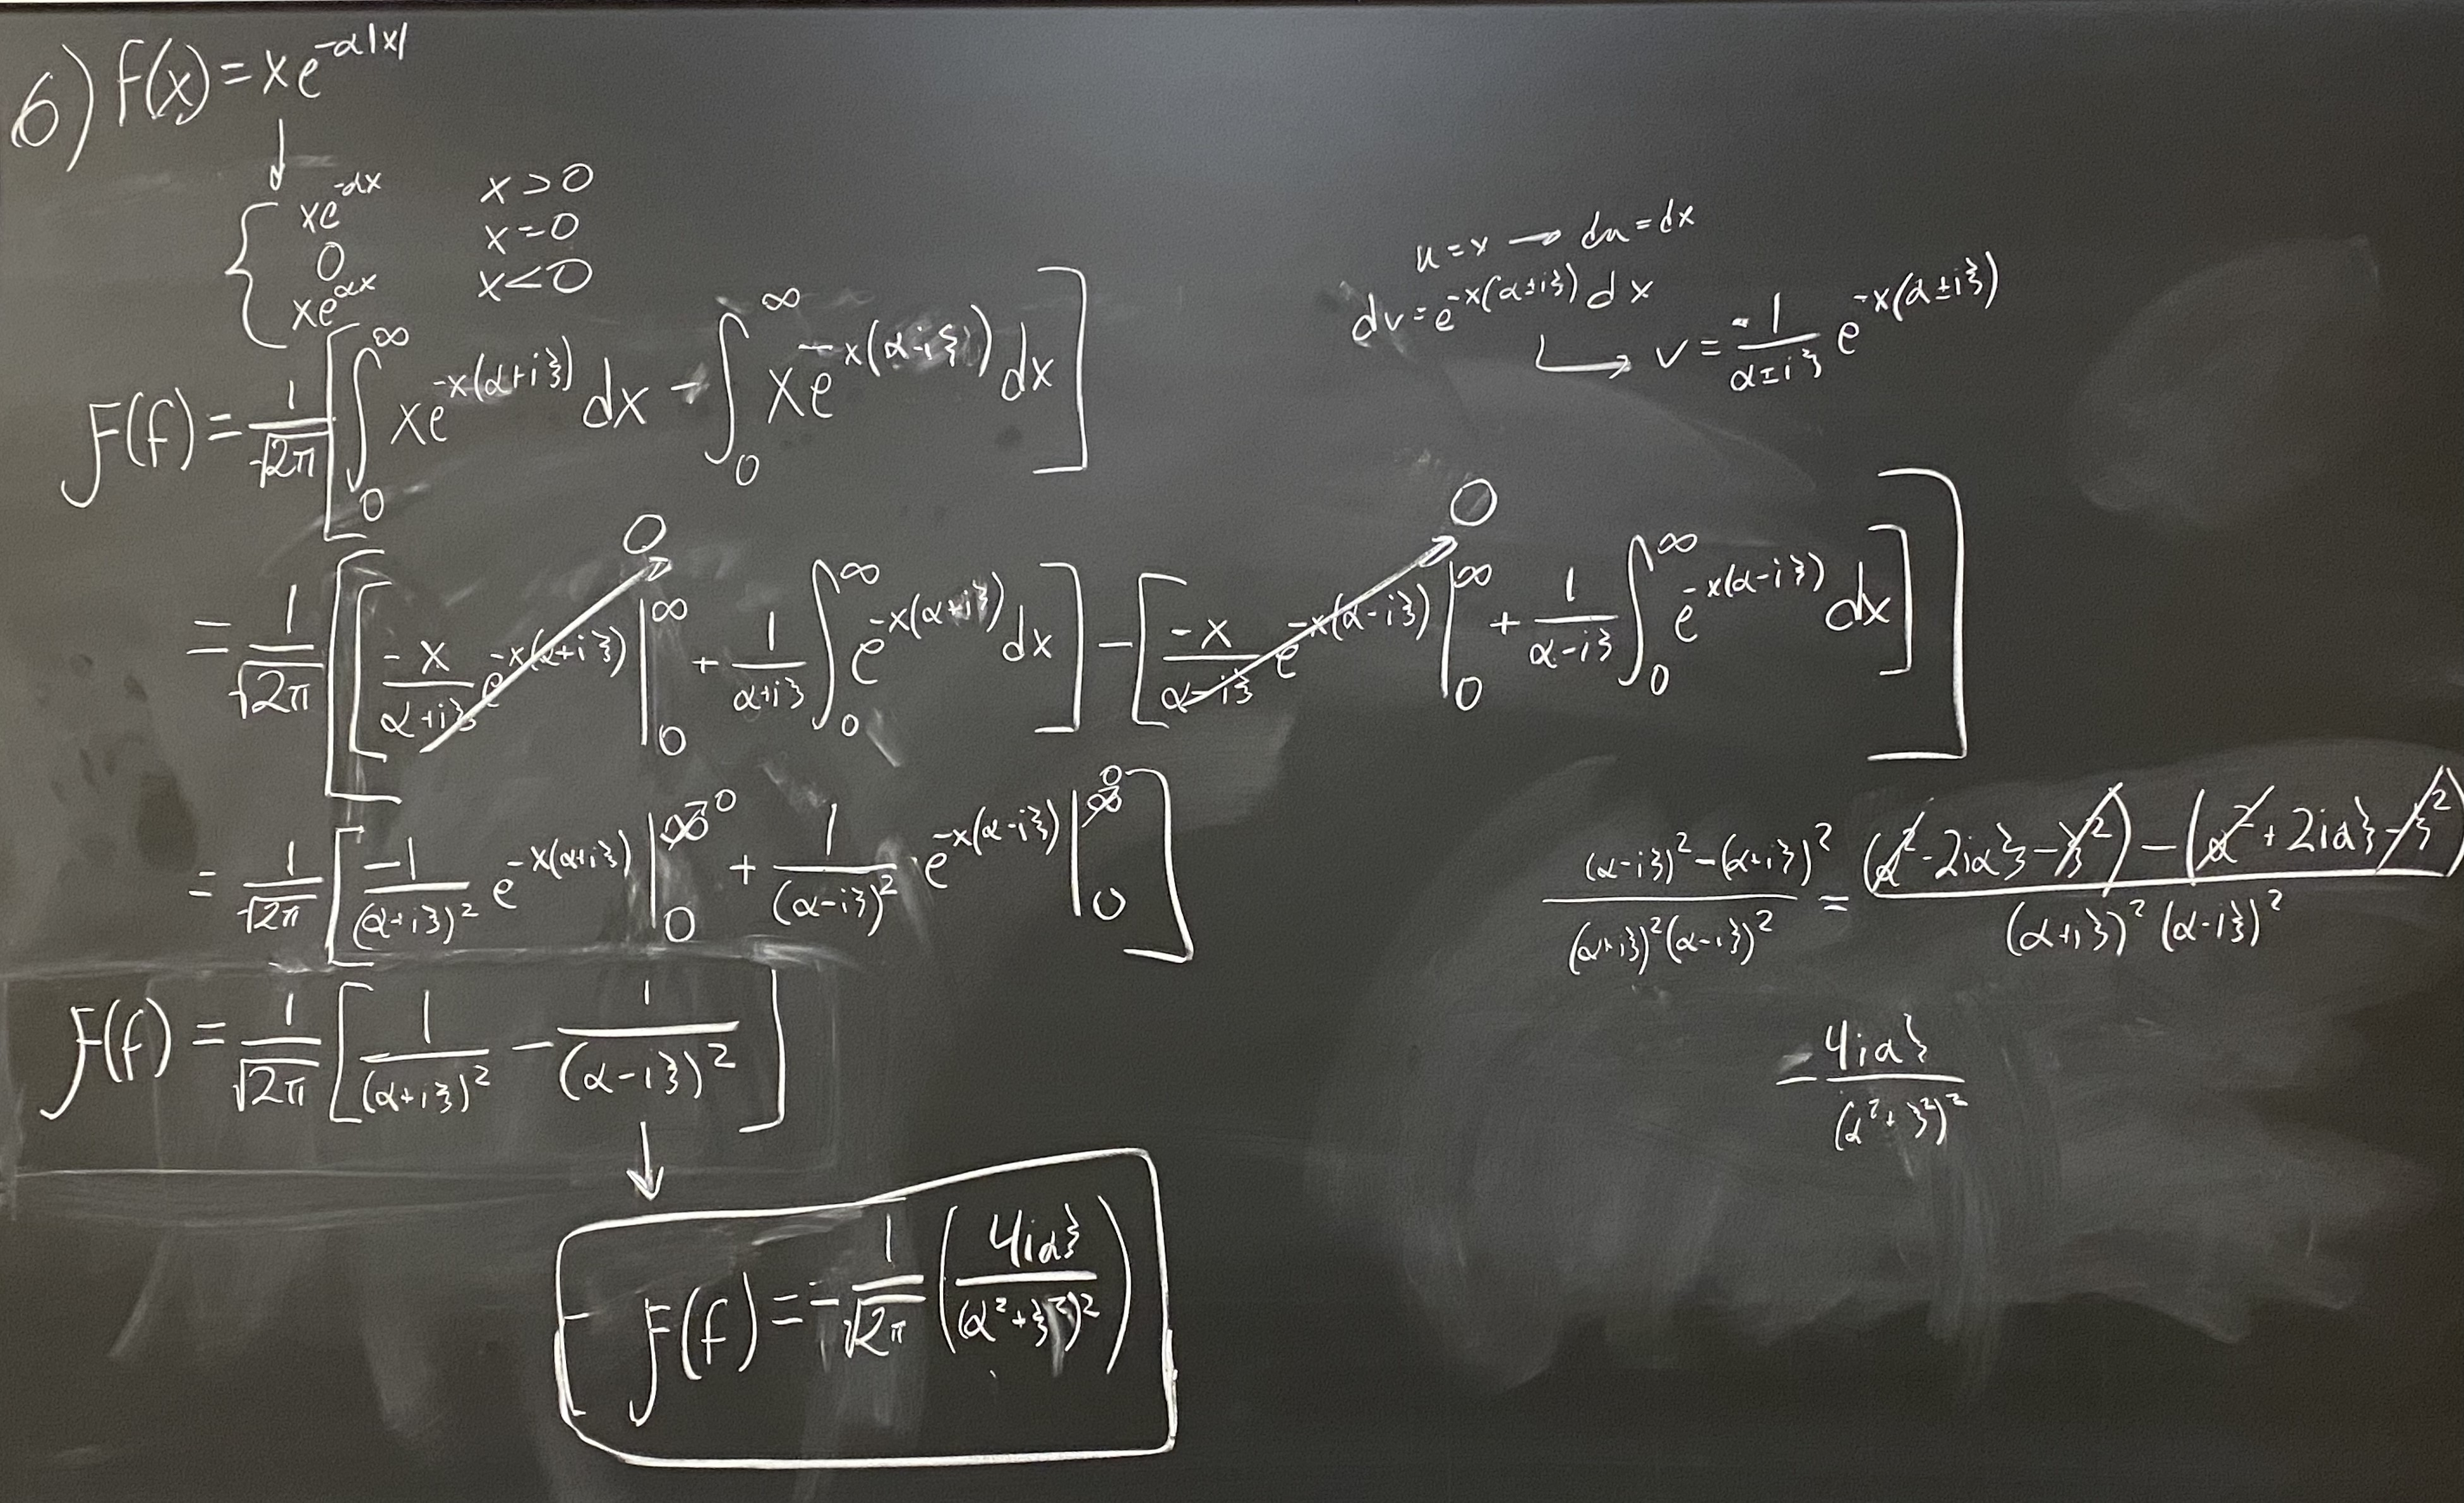
\includegraphics[width = 0.75\textwidth]{Problem 2 Part 6.jpeg}
        \end{figure}

        \item \phantom{.}
        \begin{figure}[H]
            \centering
            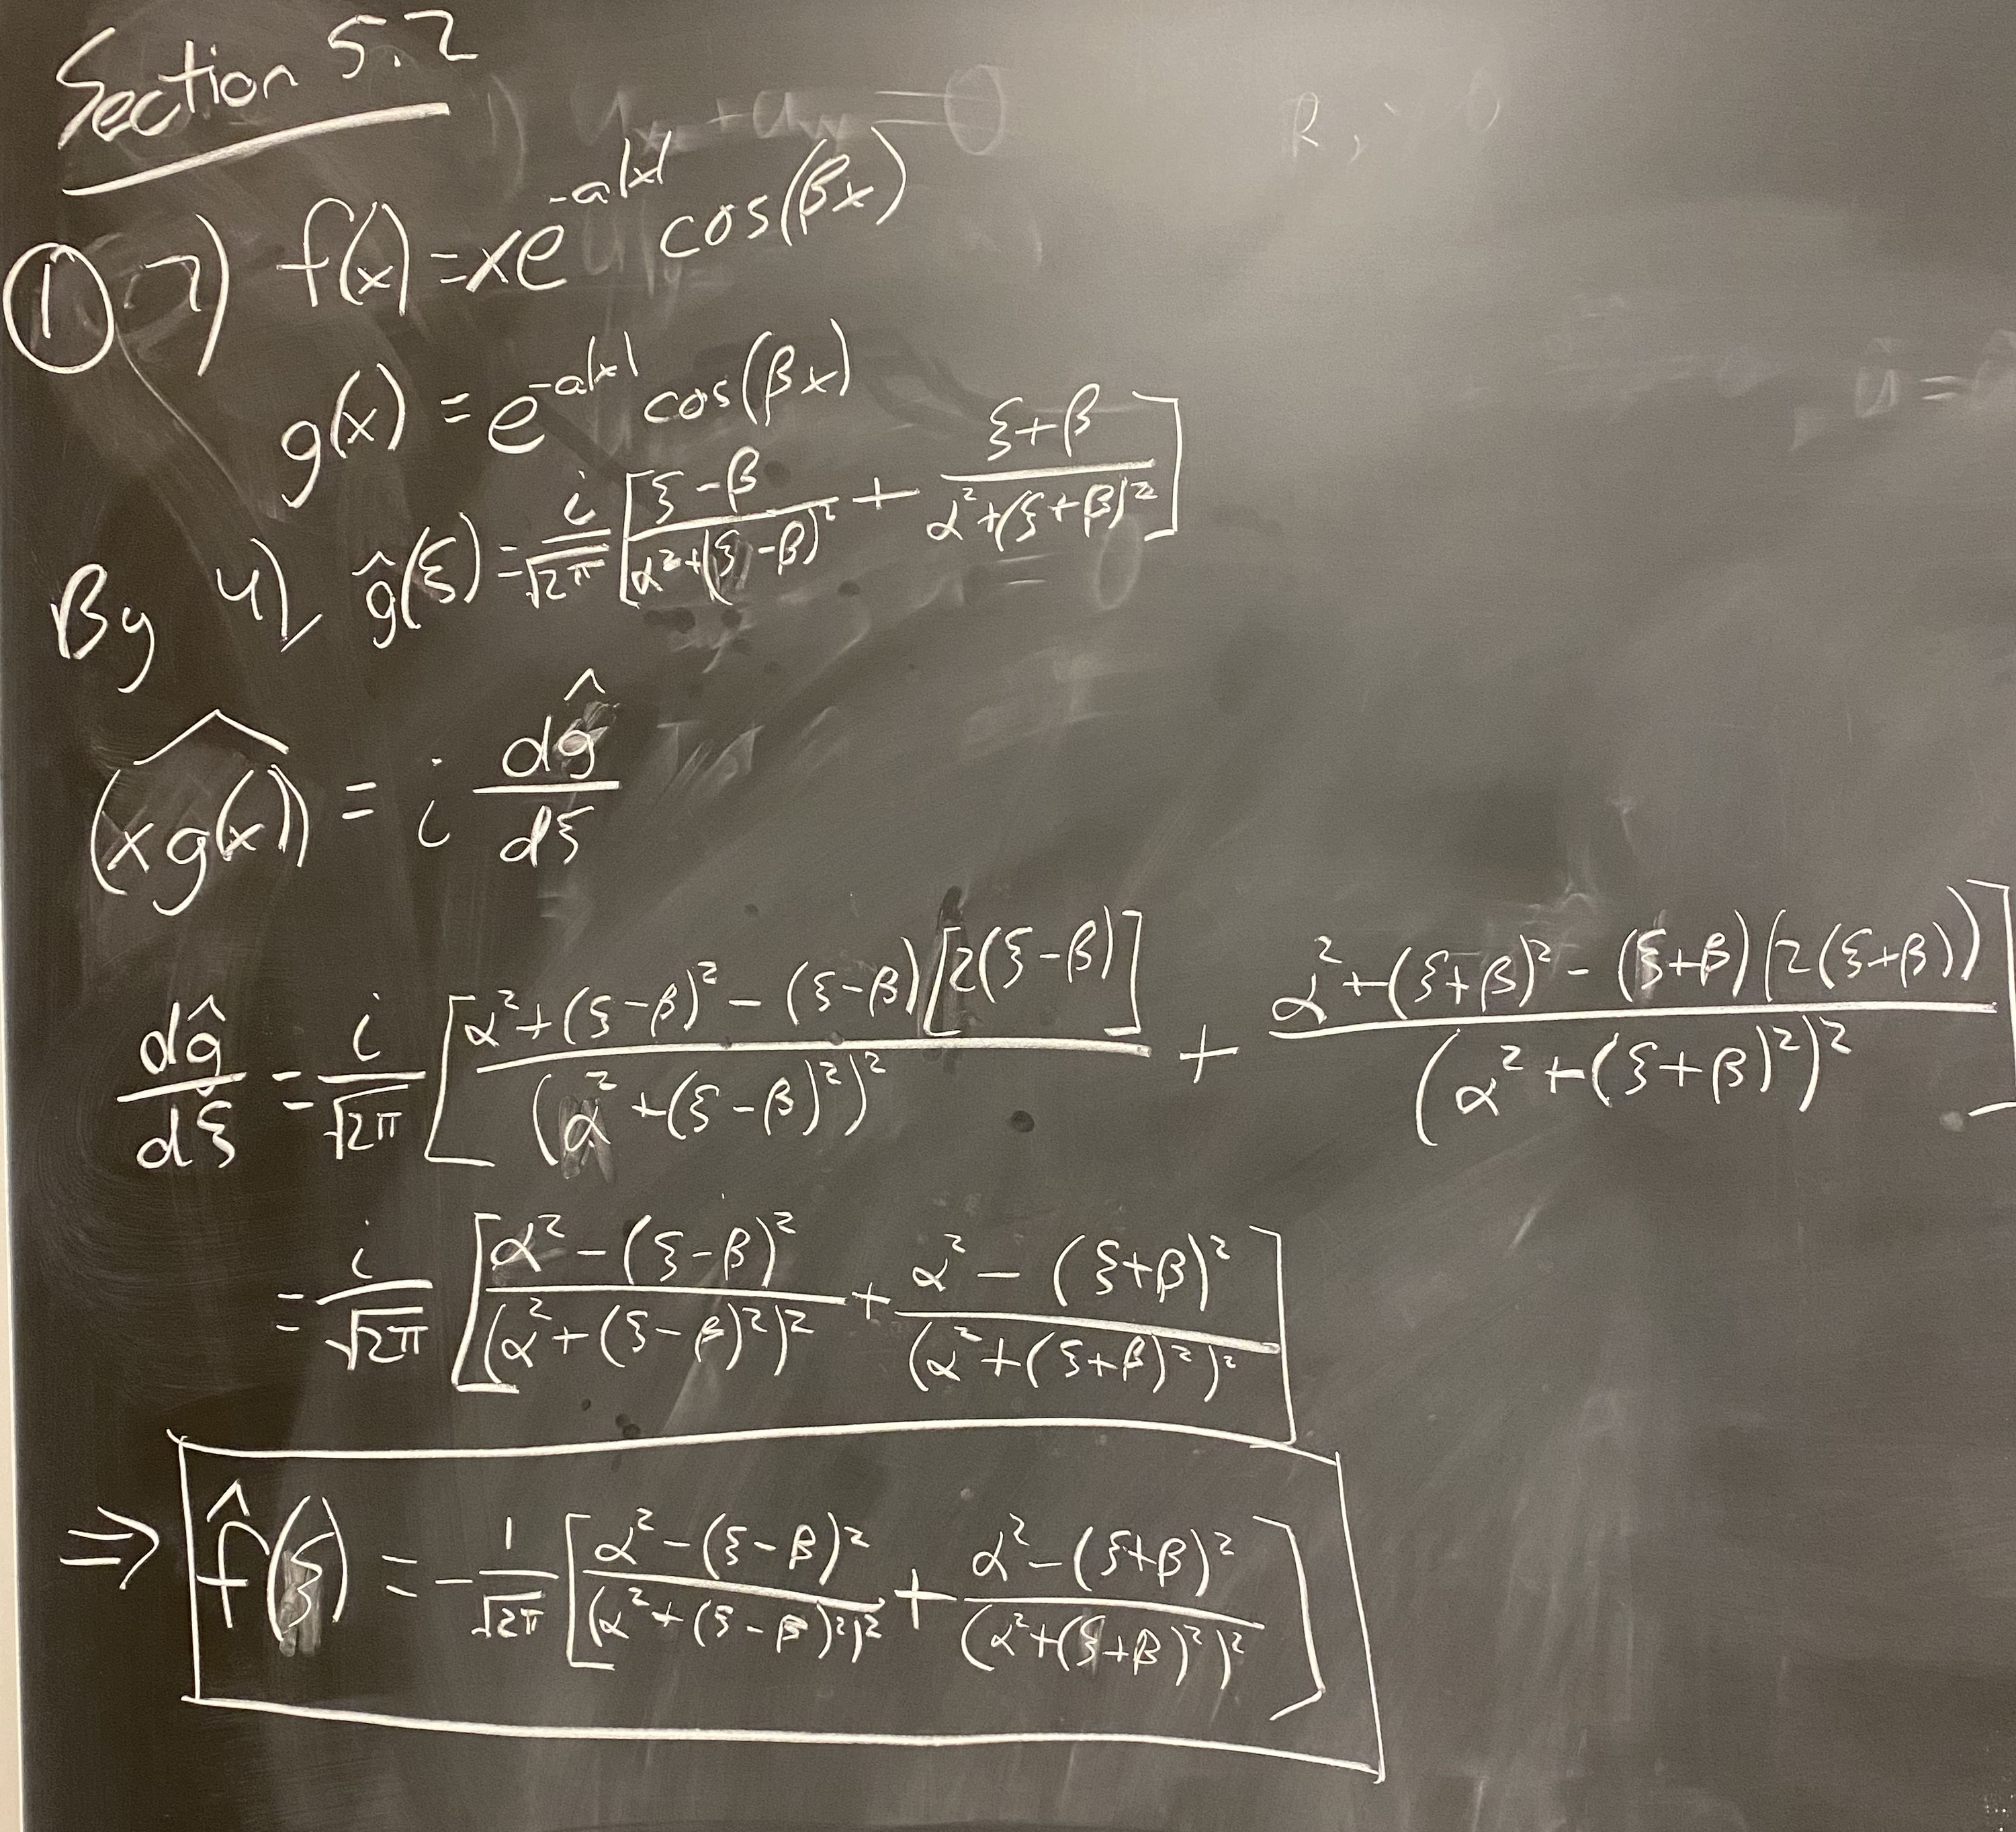
\includegraphics[width = 0.55\textwidth]{Problem 2 Part 7.jpeg}
        \end{figure}

        \item \phantom{.}
        \begin{figure}[H]
            \centering
            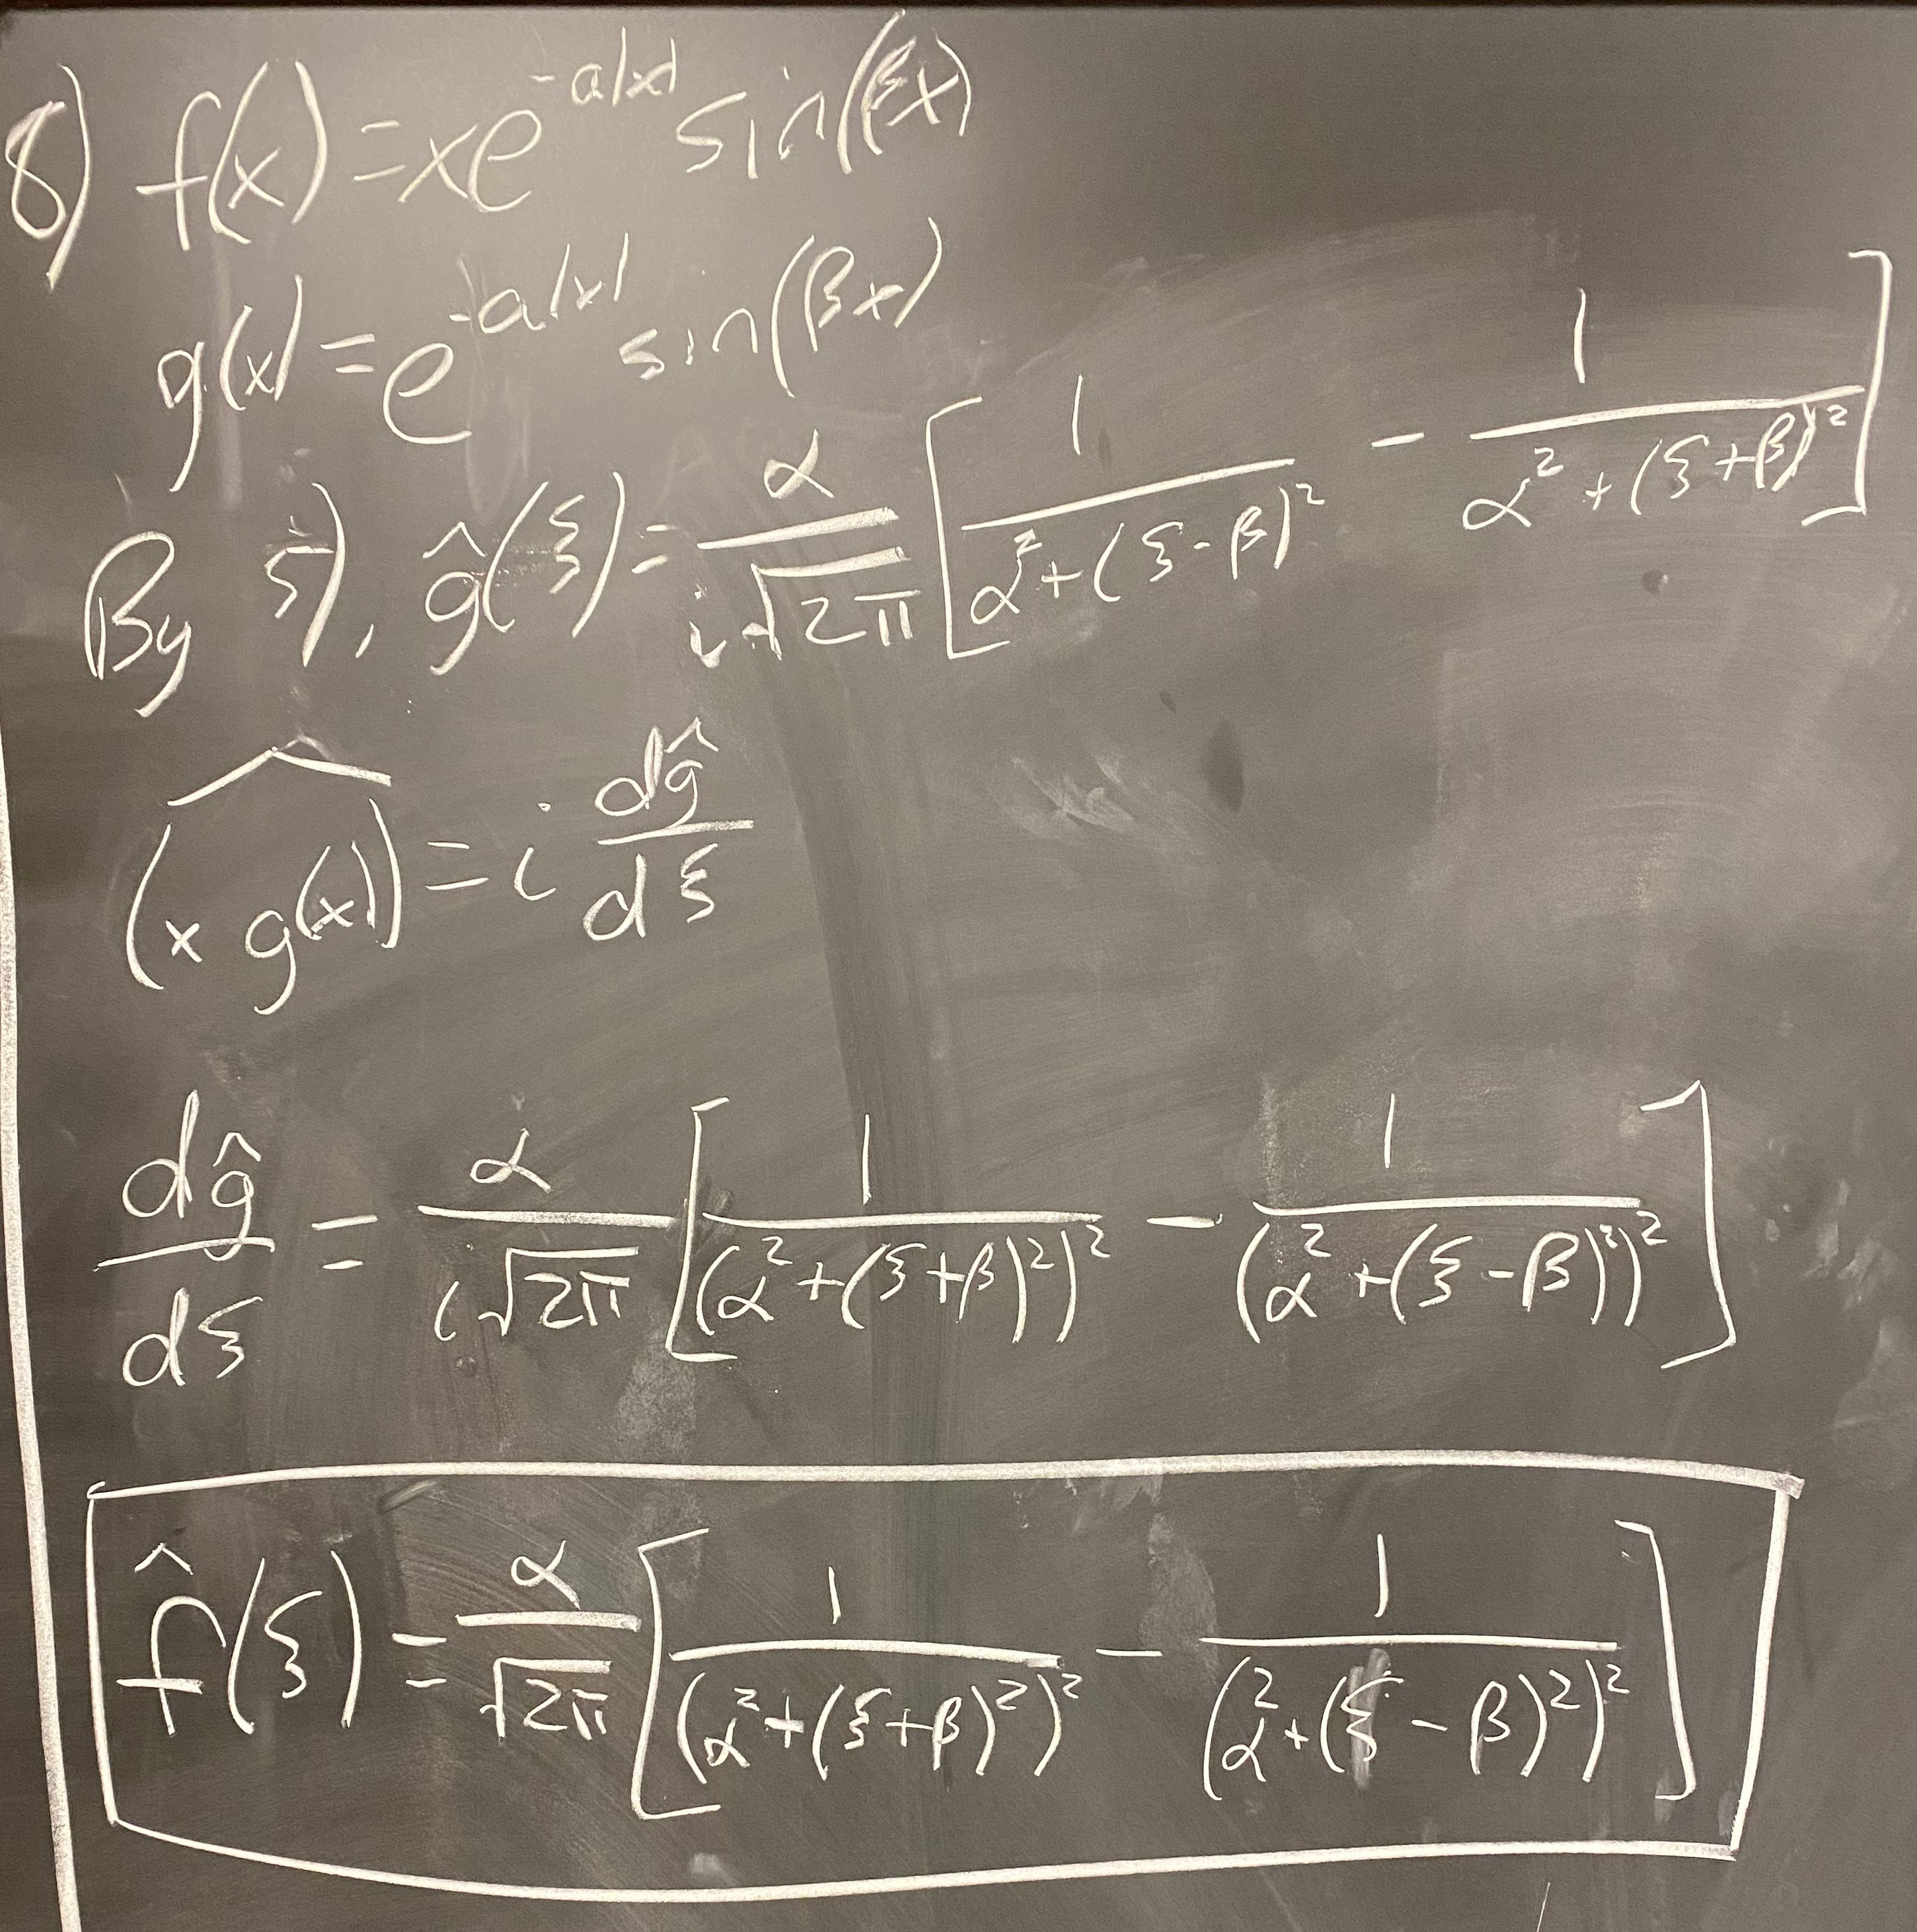
\includegraphics[width = 0.65\textwidth]{Problem 2 Part 8.jpeg}
        \end{figure}

        \item\phantom{.}
        \begin{figure}[H]
            \centering
            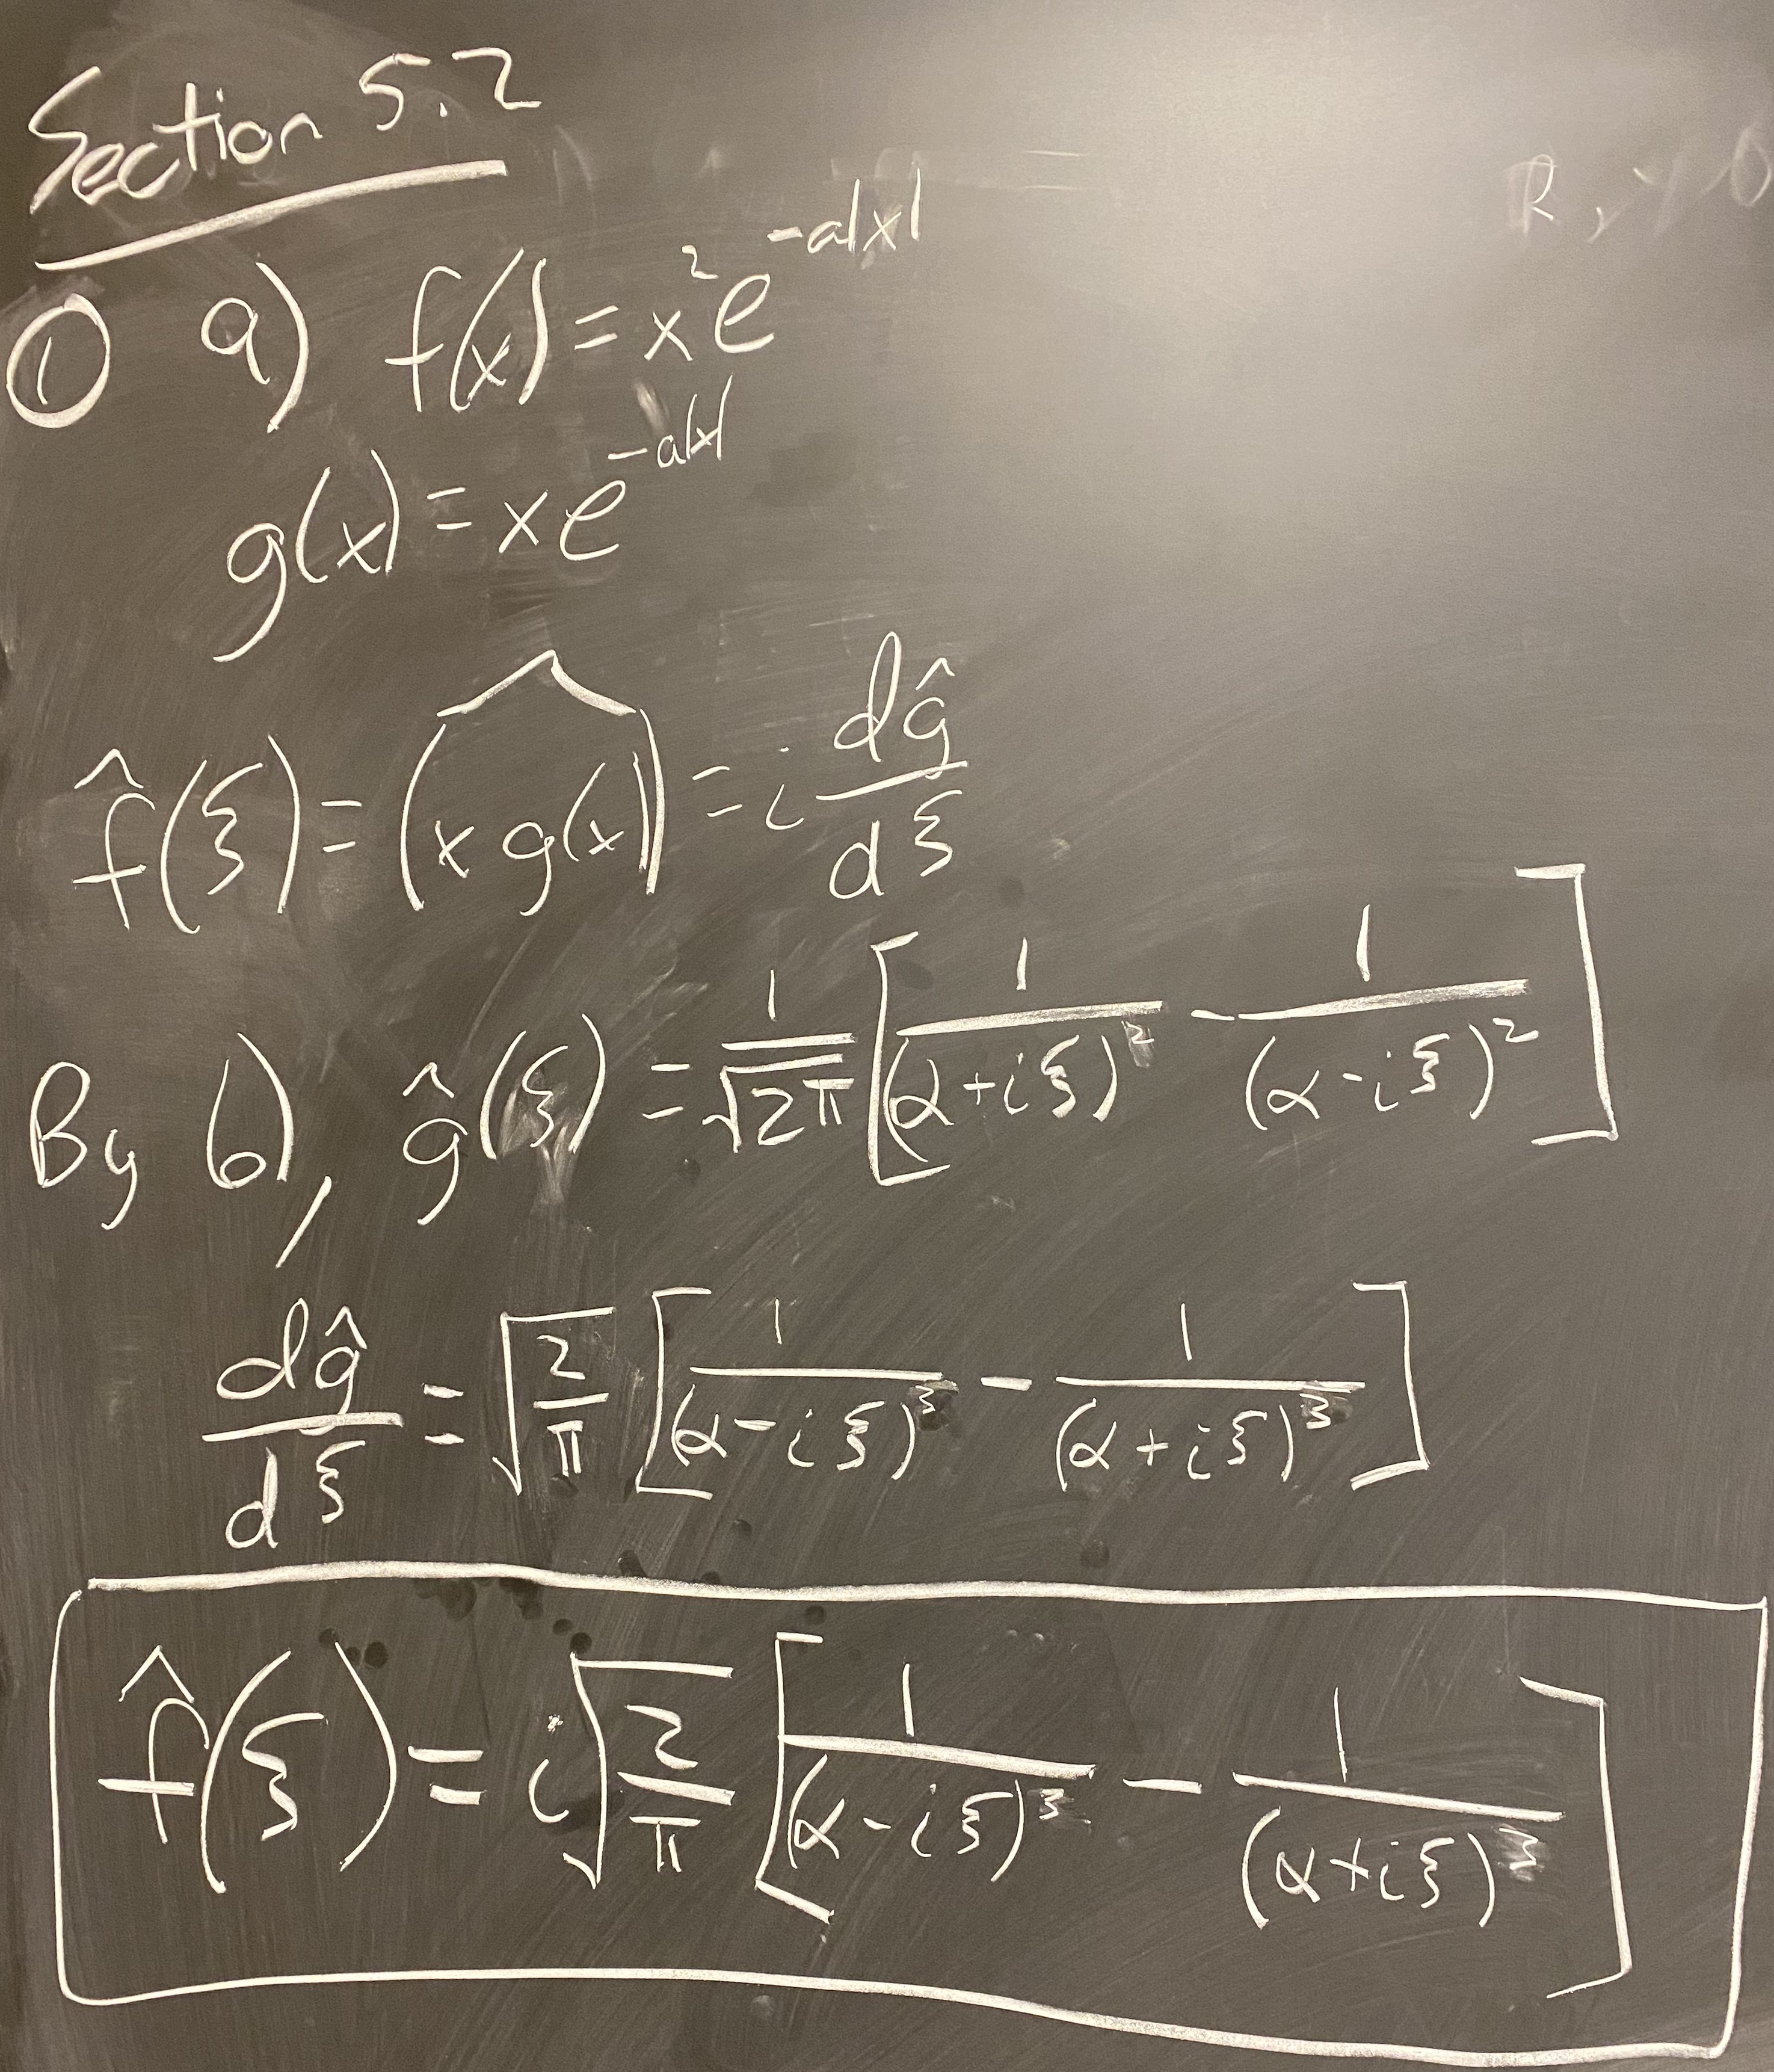
\includegraphics[width = 0.65\textwidth]{Problem 2 Part 9.jpeg}
        \end{figure}
    \end{enumerate}
\end{ans}

\begin{boldenv}
    \underline{Problem 4}. Based on Fourier transform of $e^{-\frac{\alpha x^2}{2}}$ find Fourier transforms $\hat{f}(k)$ of functions \begin{align}
        & f(x) = x e^{-\frac{\alpha x^2}{2}}\\
        & f(x) = x^2 e^{-\frac{\alpha x^2}{2}}\\
        & f(x) = e^{-\frac{\alpha x^2}{2}} \cos(\beta x)\\
        & f(x) = e^{-\frac{\alpha x^2}{2}} \sin(\beta x)\\
        & f(x) = x e^{-\frac{\alpha x^2}{2}} \cos(\beta x)\\
        & f(x) = x e^{-\frac{\alpha x^2}{2}} \sin(\beta x)
    \end{align}
\end{boldenv}
\begin{ans}
    \begin{enumerate}
        \item \phantom{.}
        \begin{figure}[H]
            \centering
            \includegraphics[width = 0.75\textwidth]{Problem 4 part 1.jpeg}
        \end{figure}

        \item \phantom{.}
        \begin{figure}[H]
            \centering
            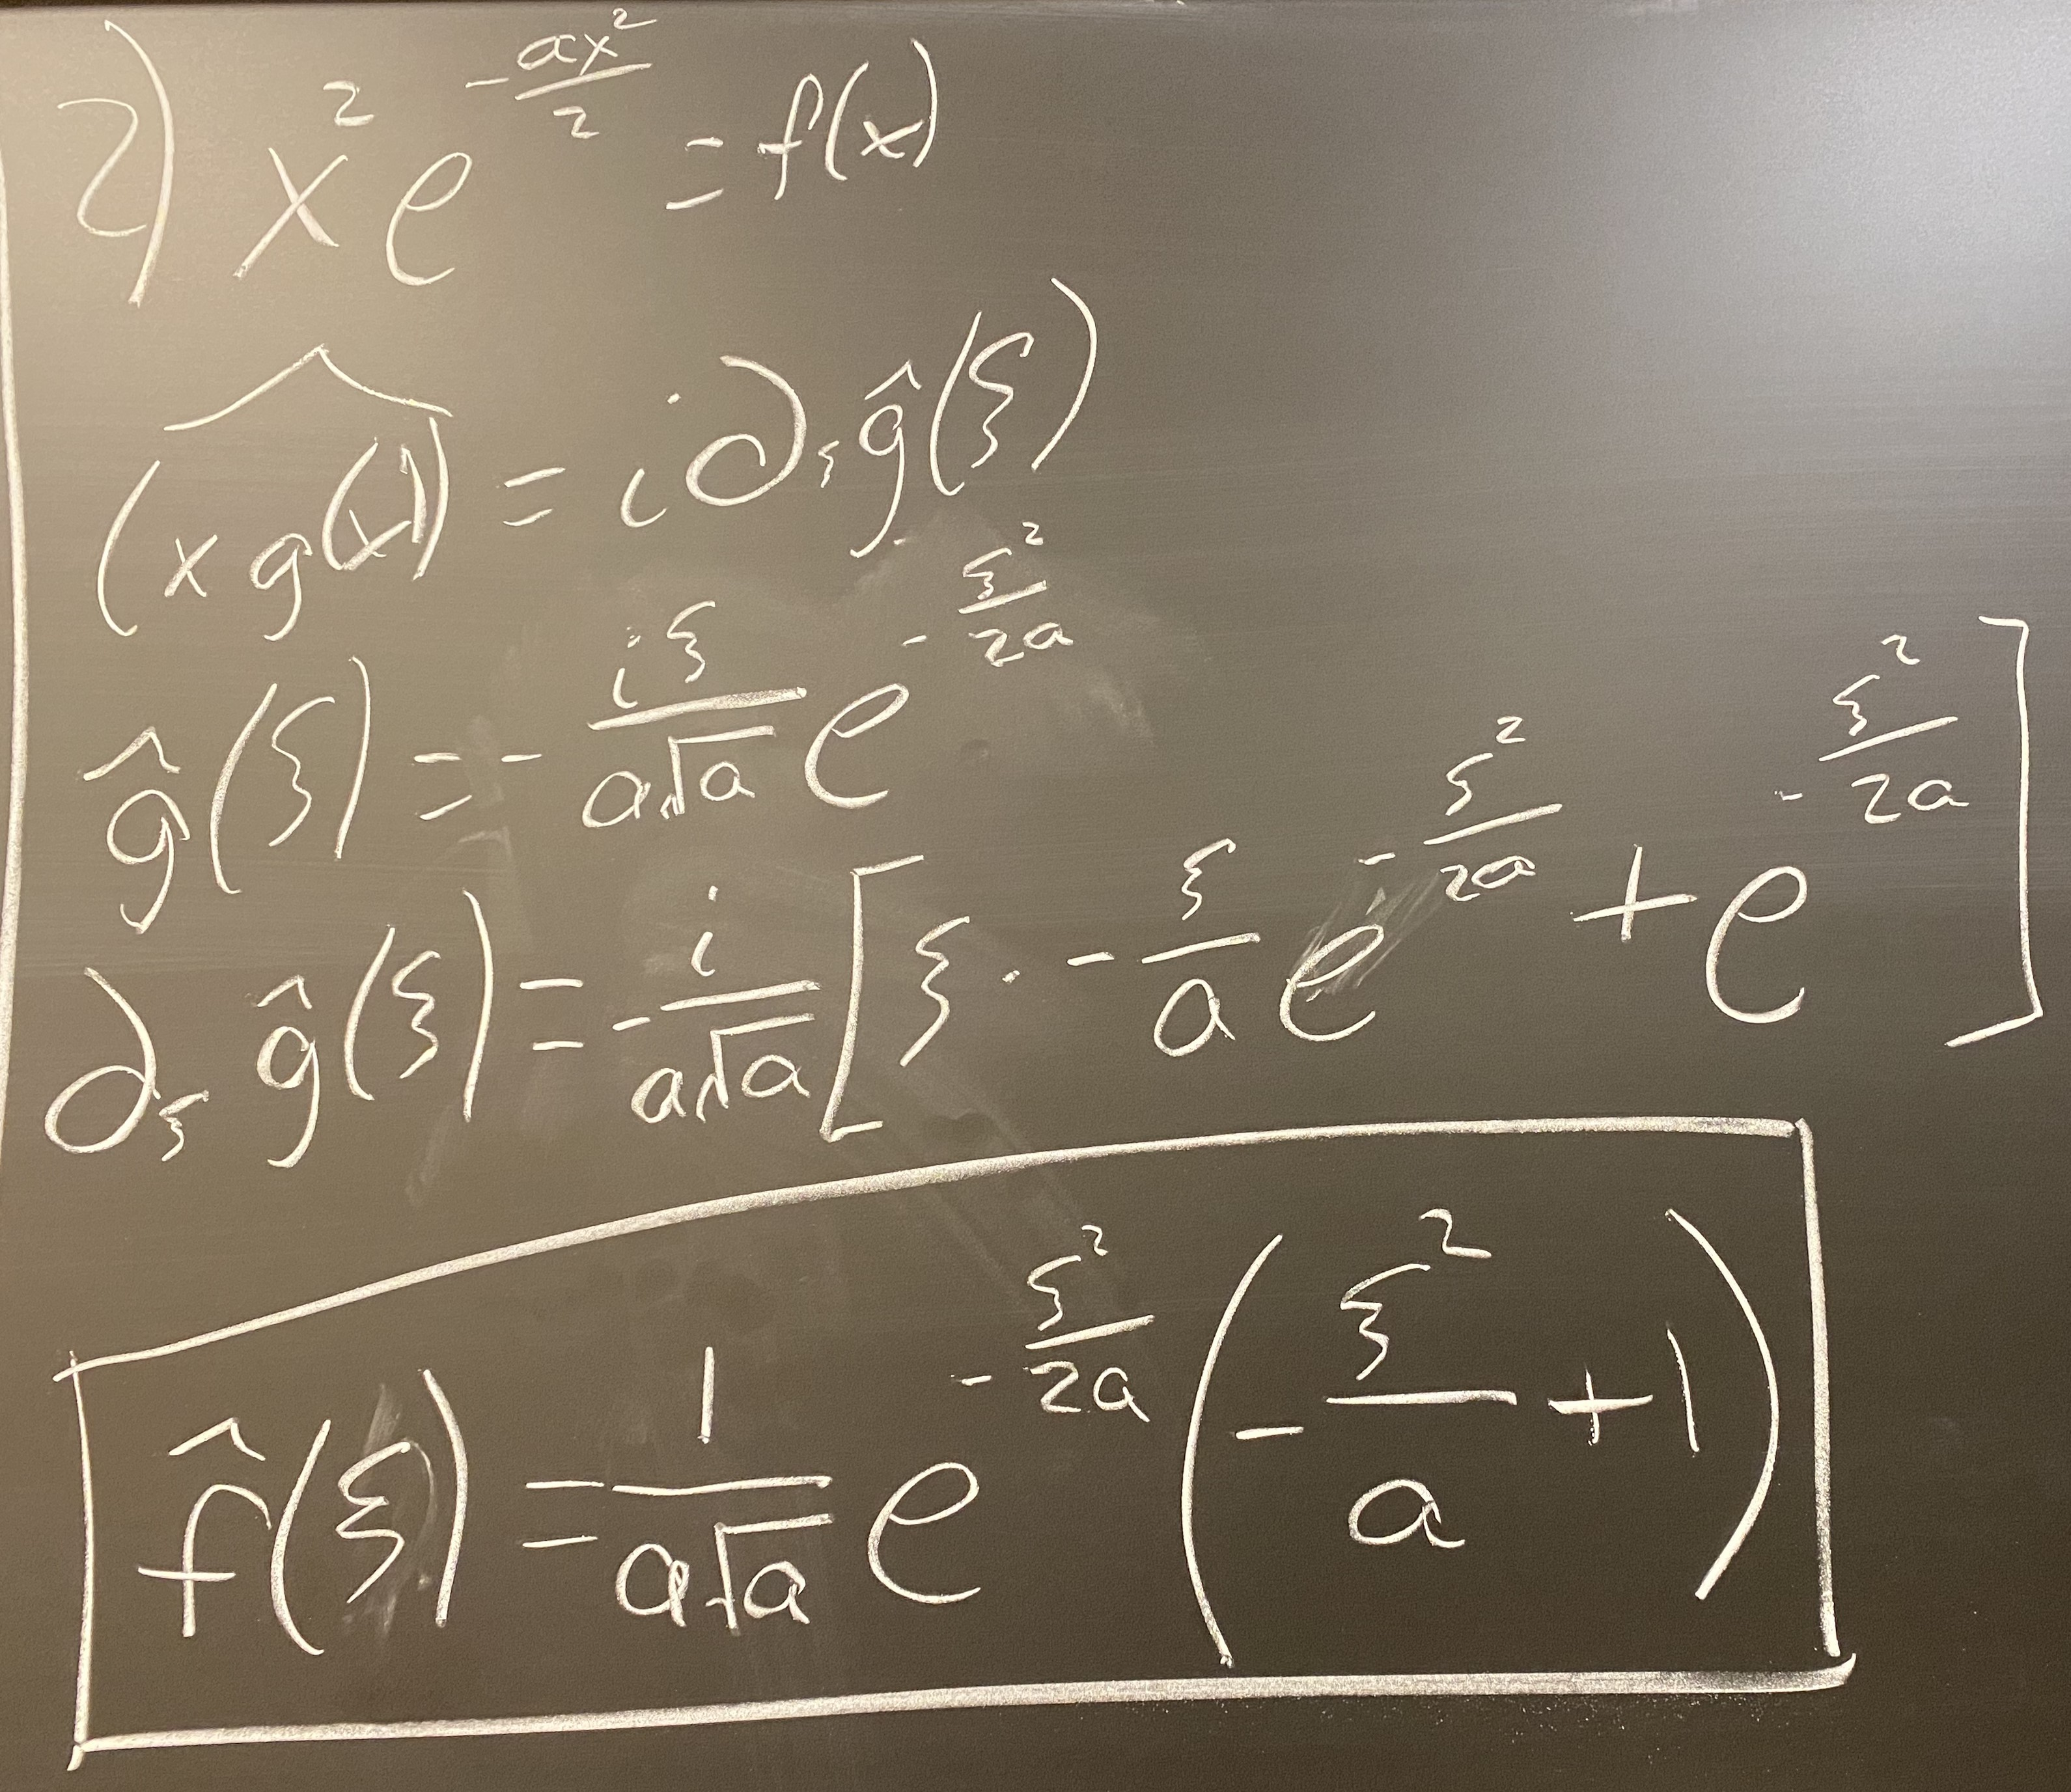
\includegraphics[width = 0.55\textwidth]{Problem 4 Part 2.jpeg}
        \end{figure}

        \item \phantom{.}
        \begin{figure}[H]
            \centering
            \includegraphics[width = 0.55\textwidth]{Problem 4 part 3.jpeg}
        \end{figure}

        \item \phantom{.}
        \begin{figure}[H]
            \centering
            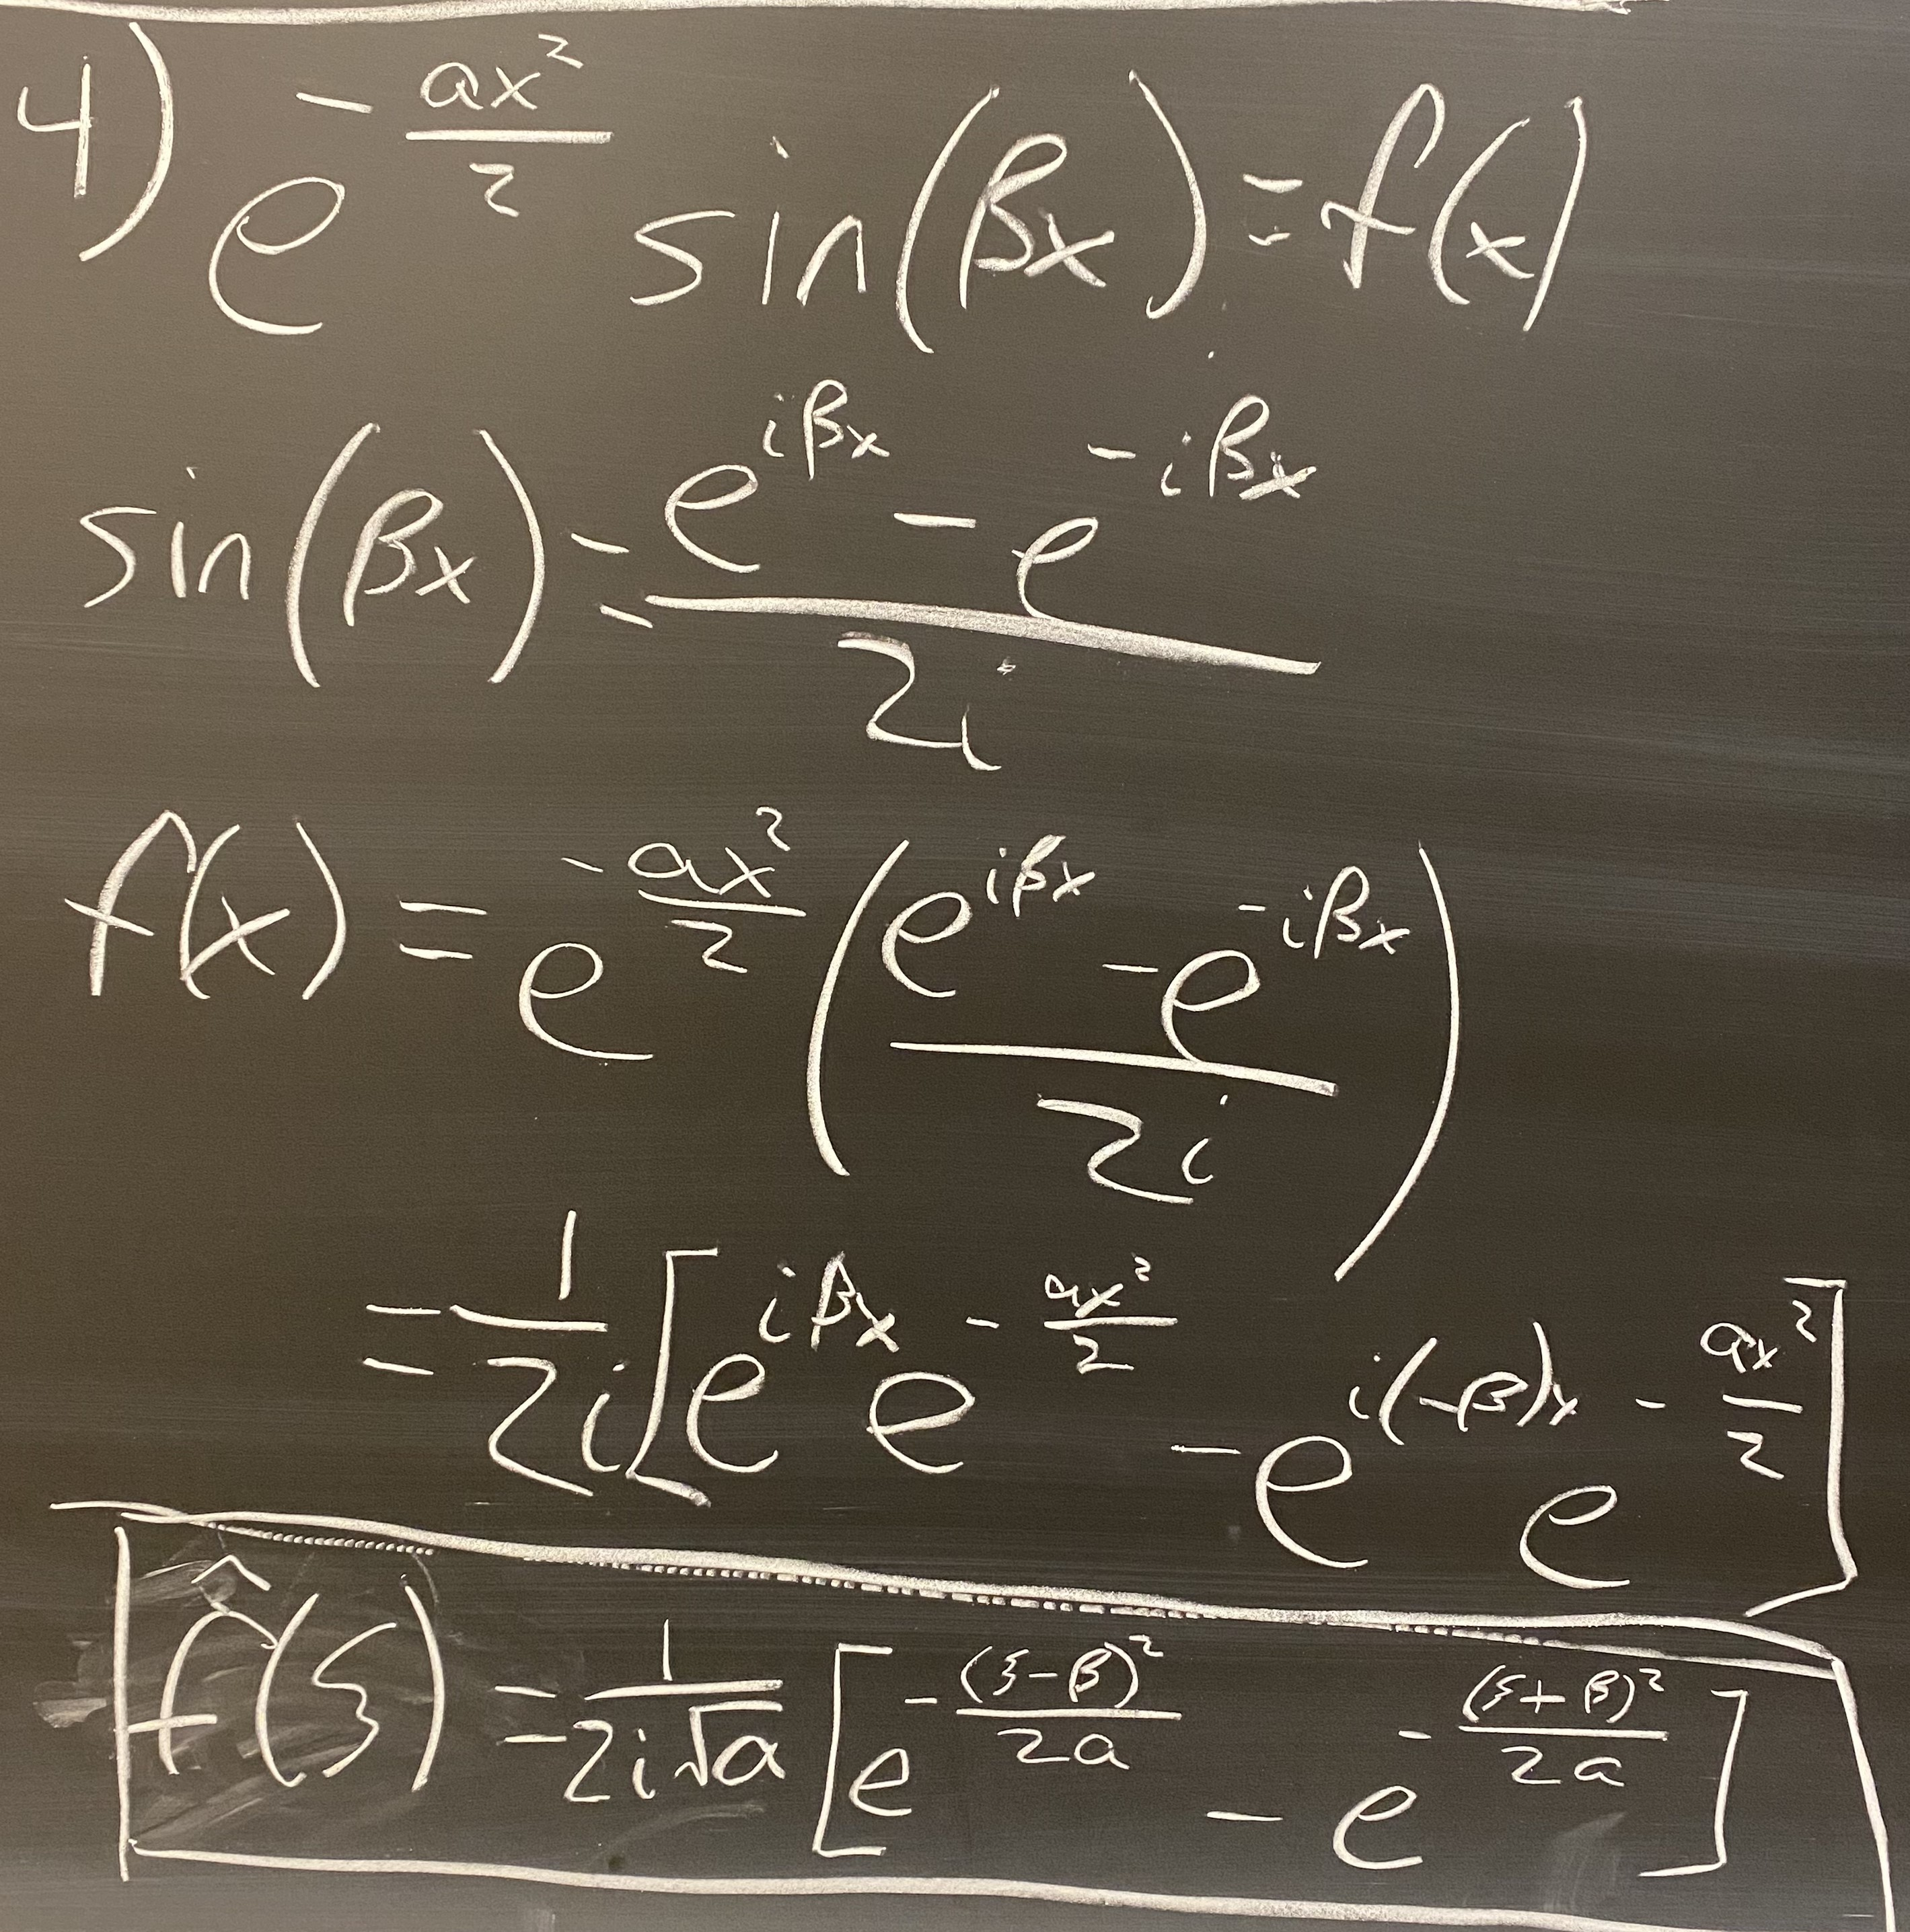
\includegraphics[width = 0.75\textwidth]{Problem 4 Part 4.jpeg}
        \end{figure}

        \item \phantom{.}
        \begin{figure}[H]
            \centering
            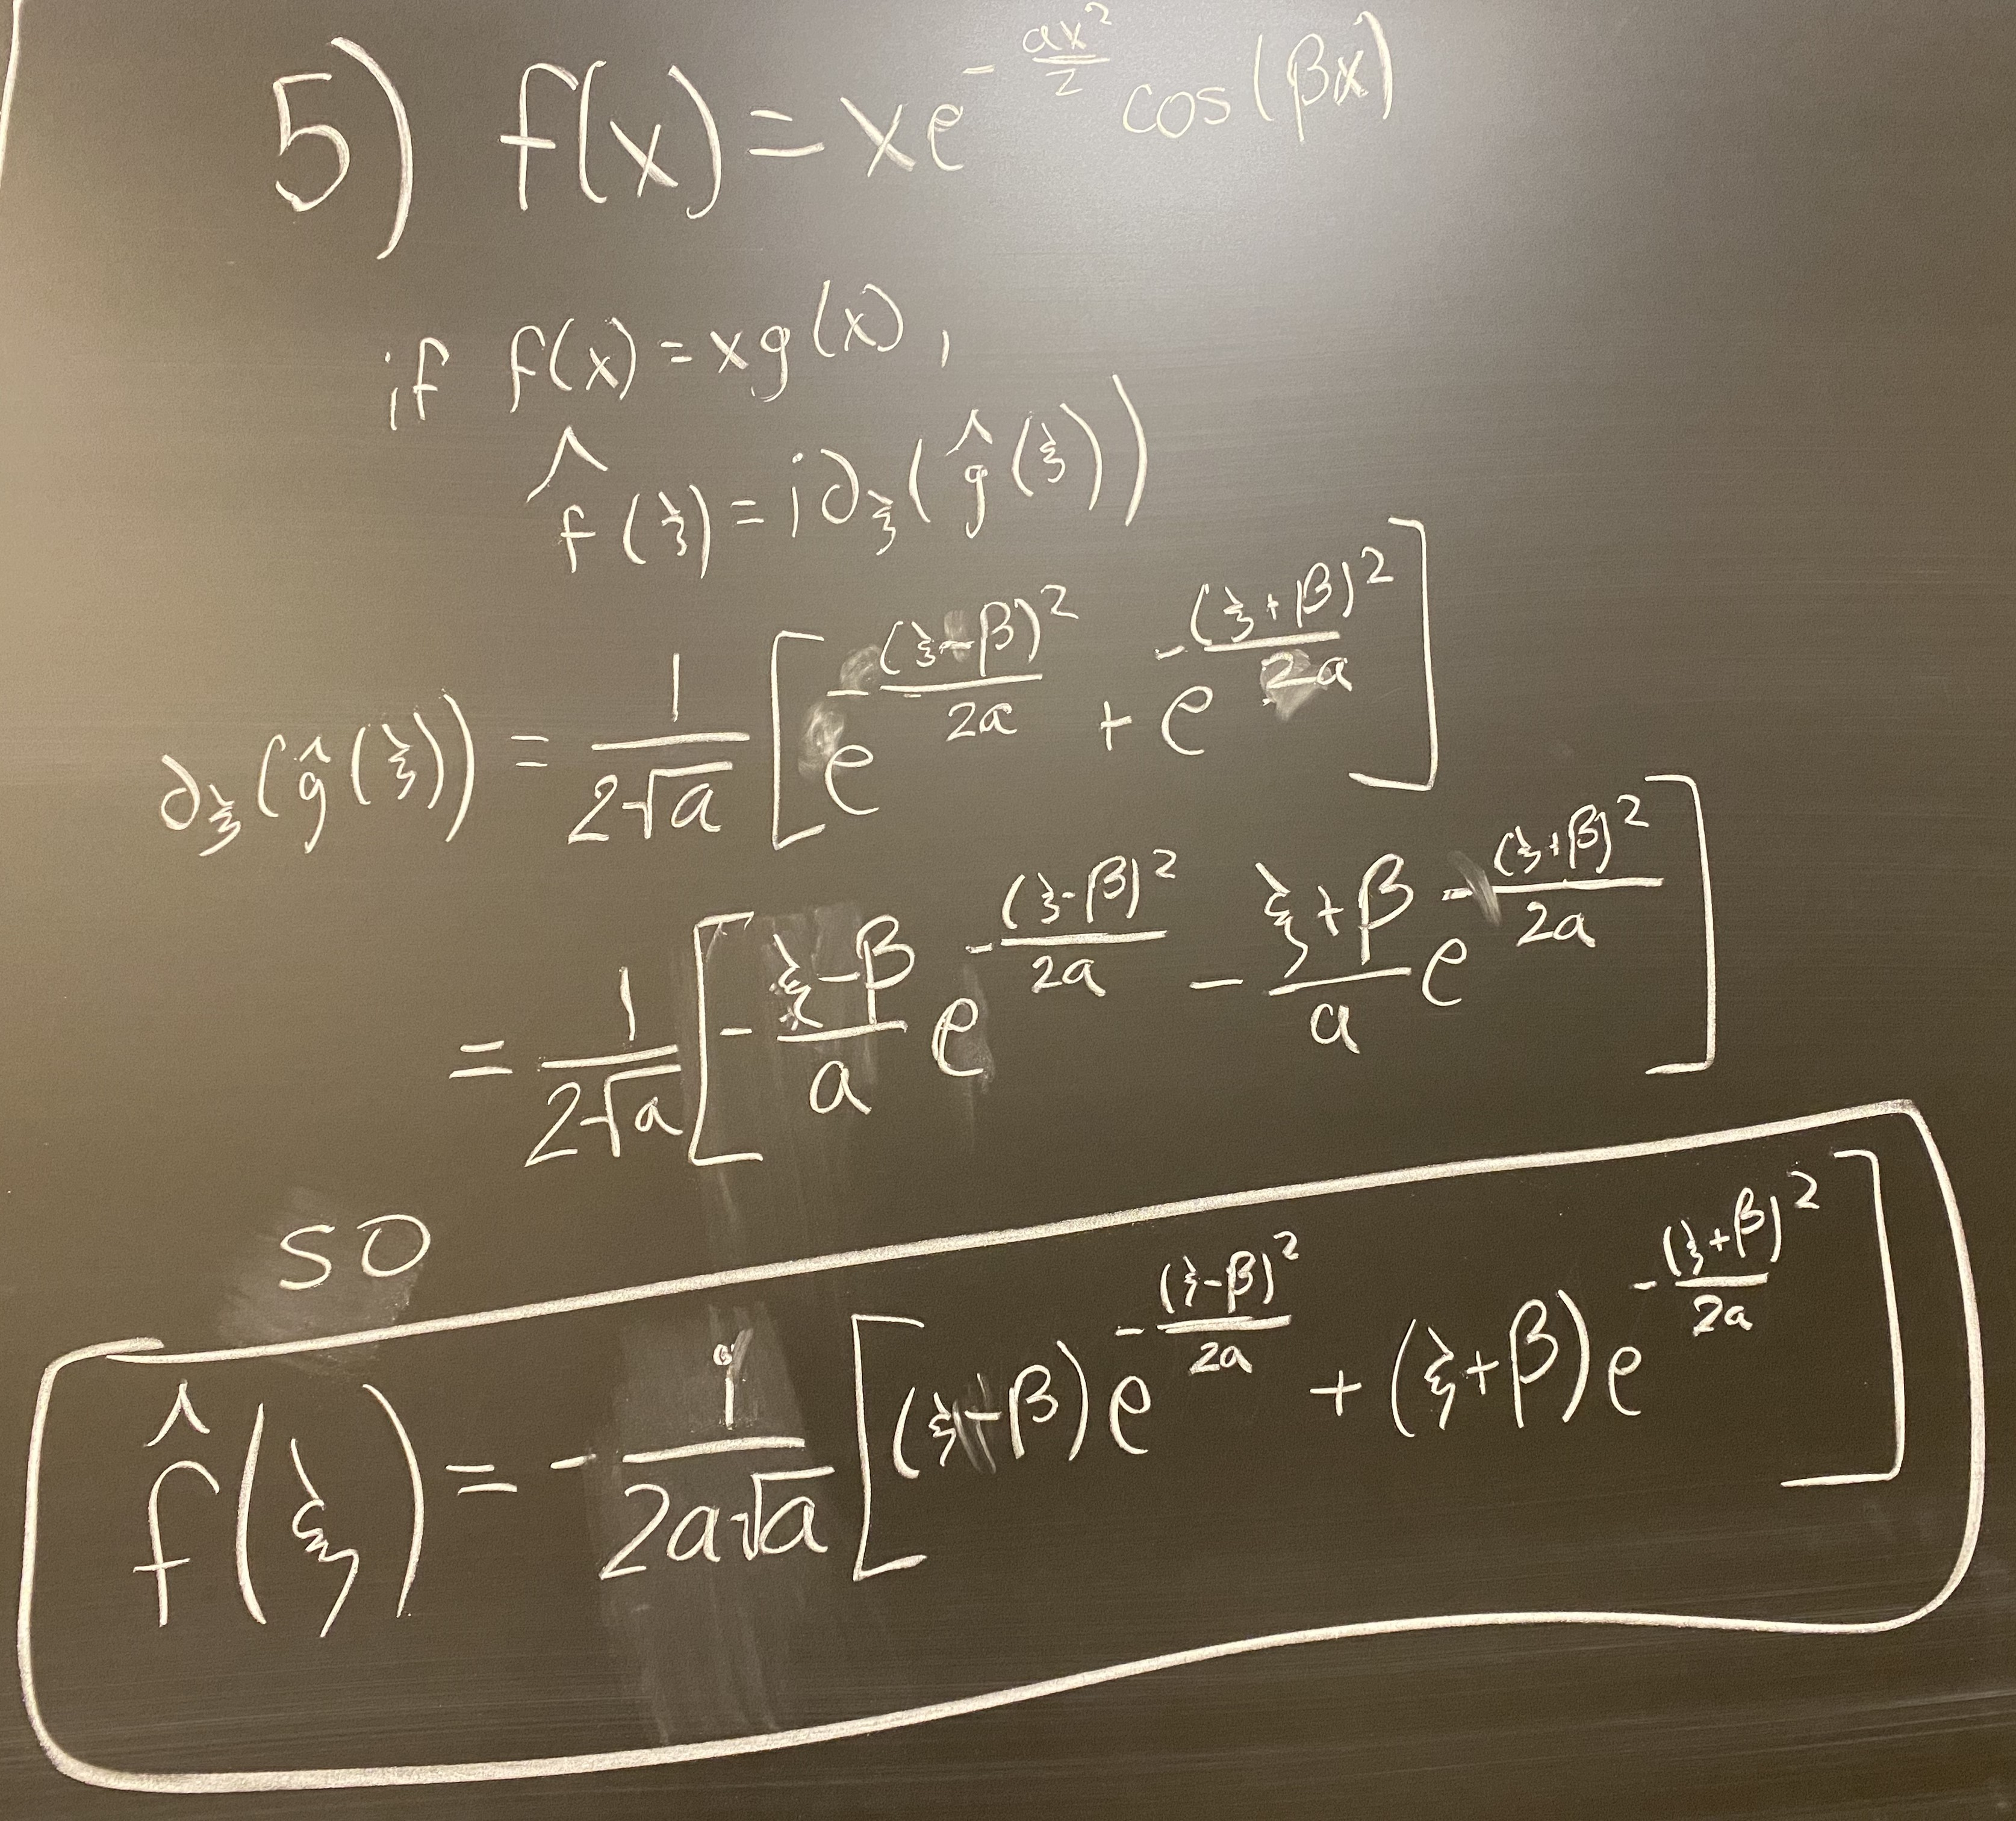
\includegraphics[width = 0.75\textwidth]{Problem 4 Part 5.jpeg}
        \end{figure}

        \item \phantom{.}
        \begin{figure}[H]
            \centering
            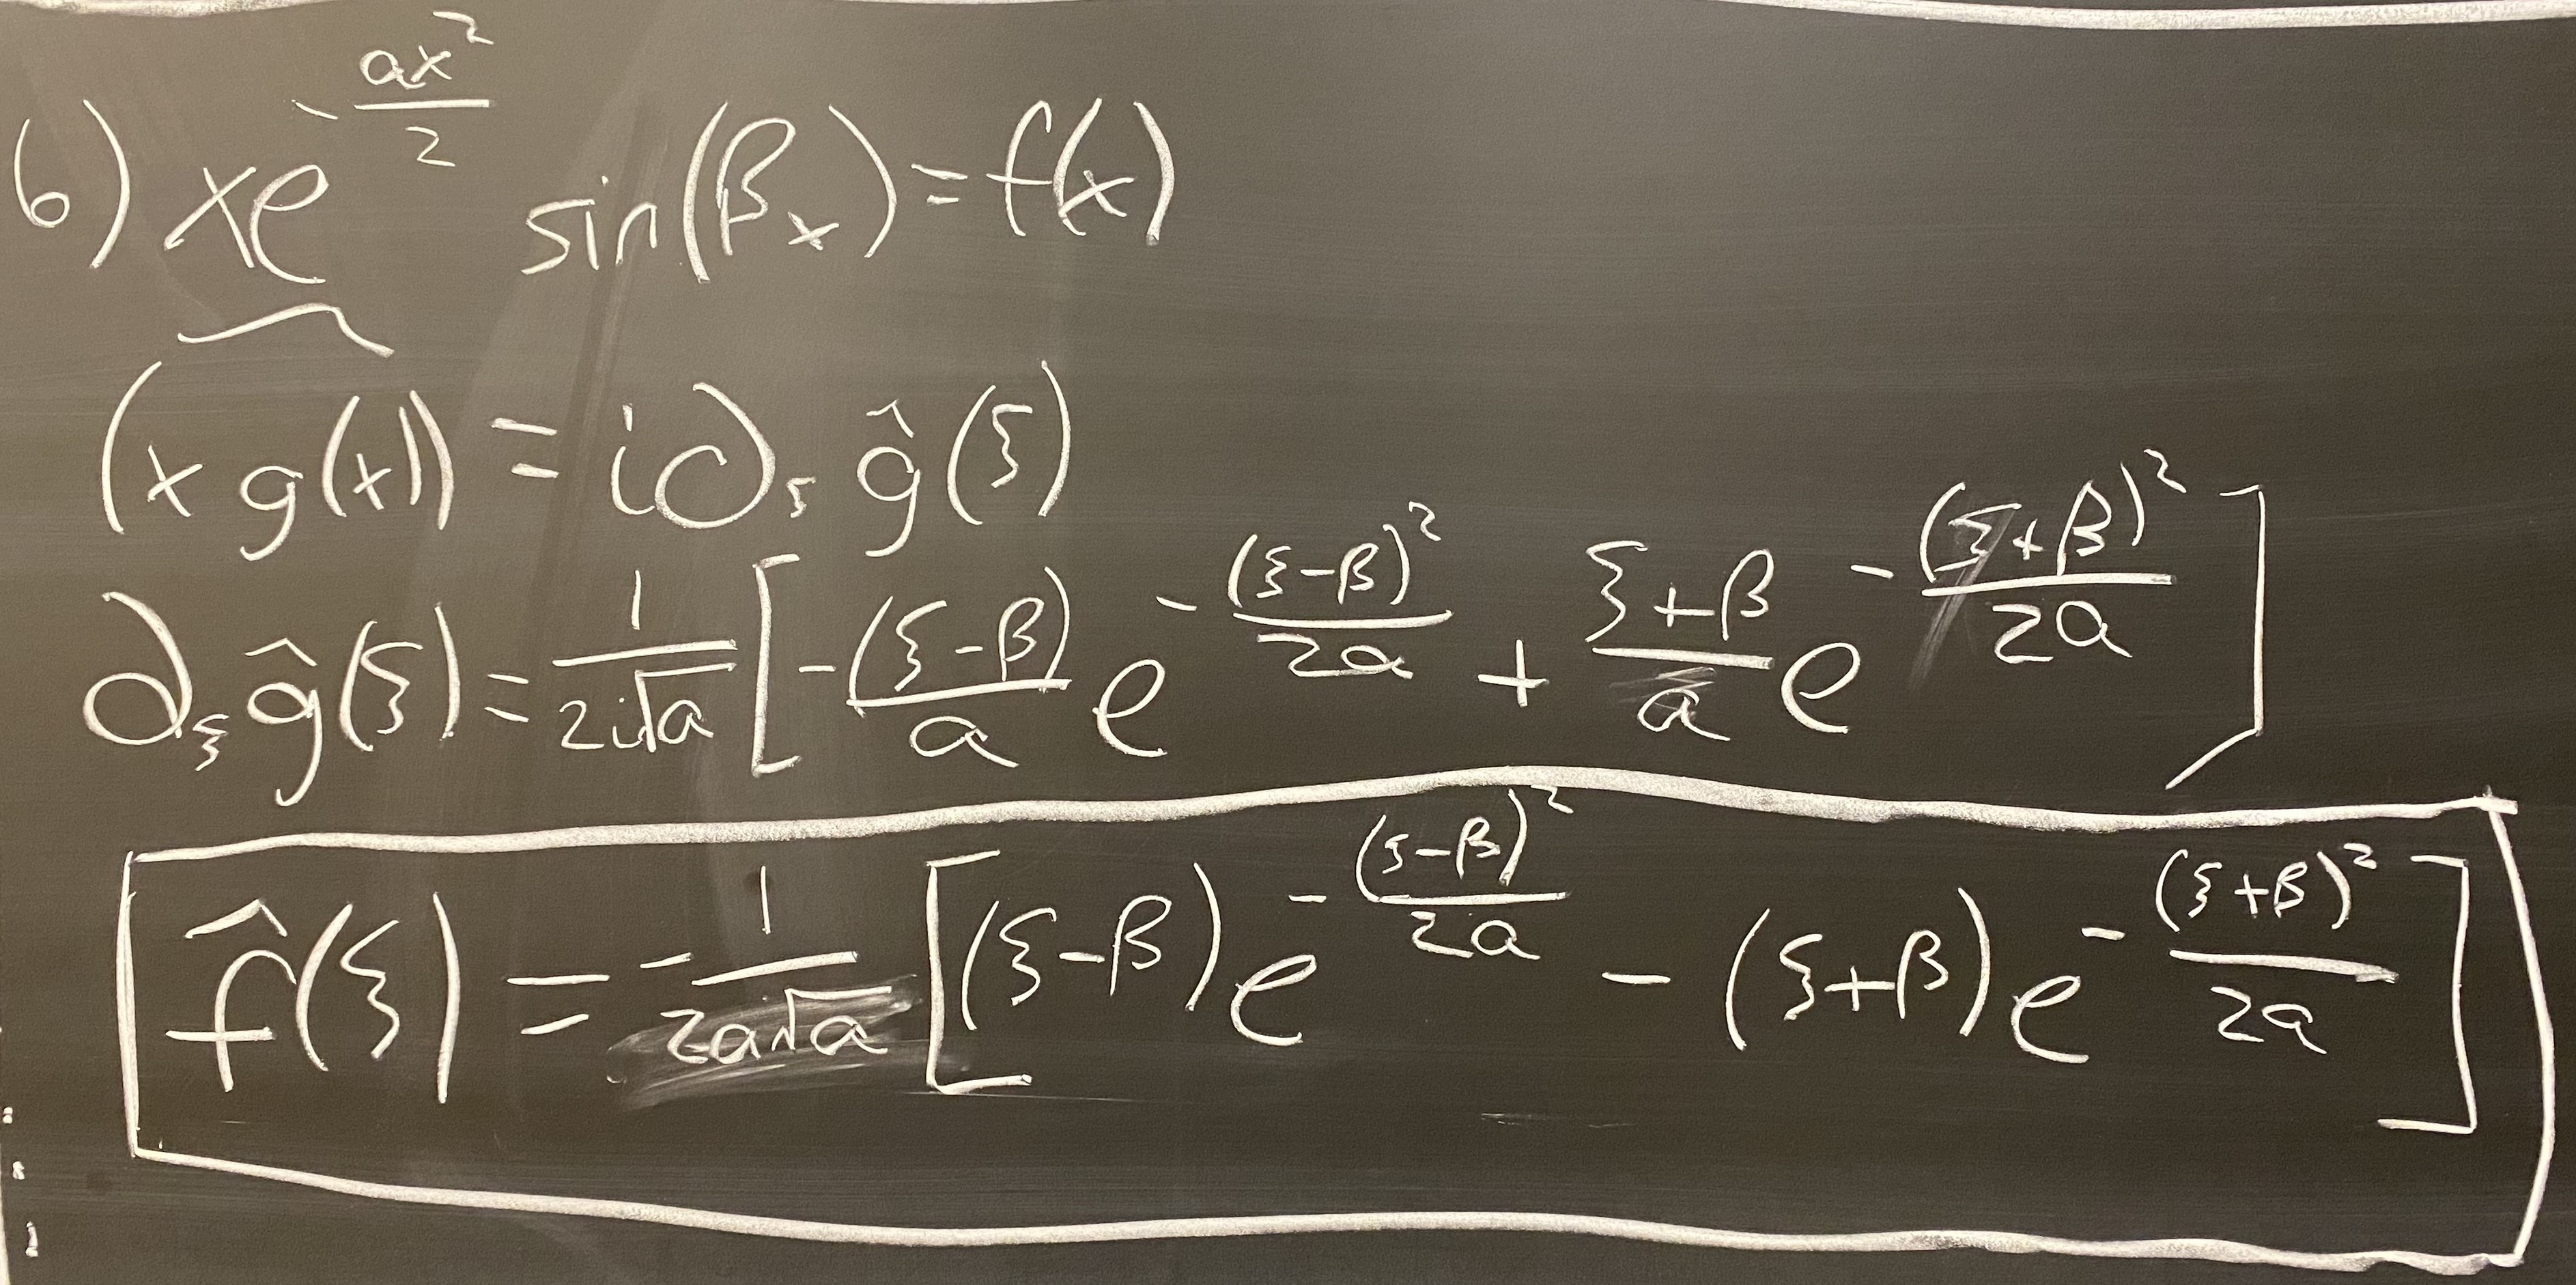
\includegraphics[width = 0.75\textwidth]{Problem 4 Part 6.jpeg}
        \end{figure}
    \end{enumerate}
\end{ans}

\begin{boldenv}
    \underline{Problem 5}. Let $a > 0$. Find Fourier transforms $\hat{f}(k)$ of functions \begin{align}
        & f(x) = \begin{cases}
            1 & \mkern 50mu |x| \leq a\\
            0 & \mkern 50mu |x| > a
        \end{cases}\\
        & f(x) = \begin{cases}
            x & \mkern 50mu |x| \leq a\\
            0 & \mkern 50mu |x| > a
        \end{cases}\\
        & f(x) = \begin{cases}
            |x| & \mkern 50mu |x| \leq a\\
            0 & \mkern 50mu |x| > a
        \end{cases}\\
        & f(x) = \begin{cases}
            a - |x| & \mkern 50mu |x| \leq a\\
            0 & \mkern 50mu |x| > a
        \end{cases}\\
        & f(x) = \begin{cases}
            a^2 - x^2 & \mkern 50mu |x| \leq a\\
            0 & \mkern 50mu |x| > a
        \end{cases}\\
        & \text{Using 1, calculate} \int_{-\infty}^\infty \frac{\sin(x)}{x}\,dx.
    \end{align}
\end{boldenv}
\begin{ans}
    \begin{enumerate}
        \item \phantom{.}
        \begin{figure}[H]
            \centering
            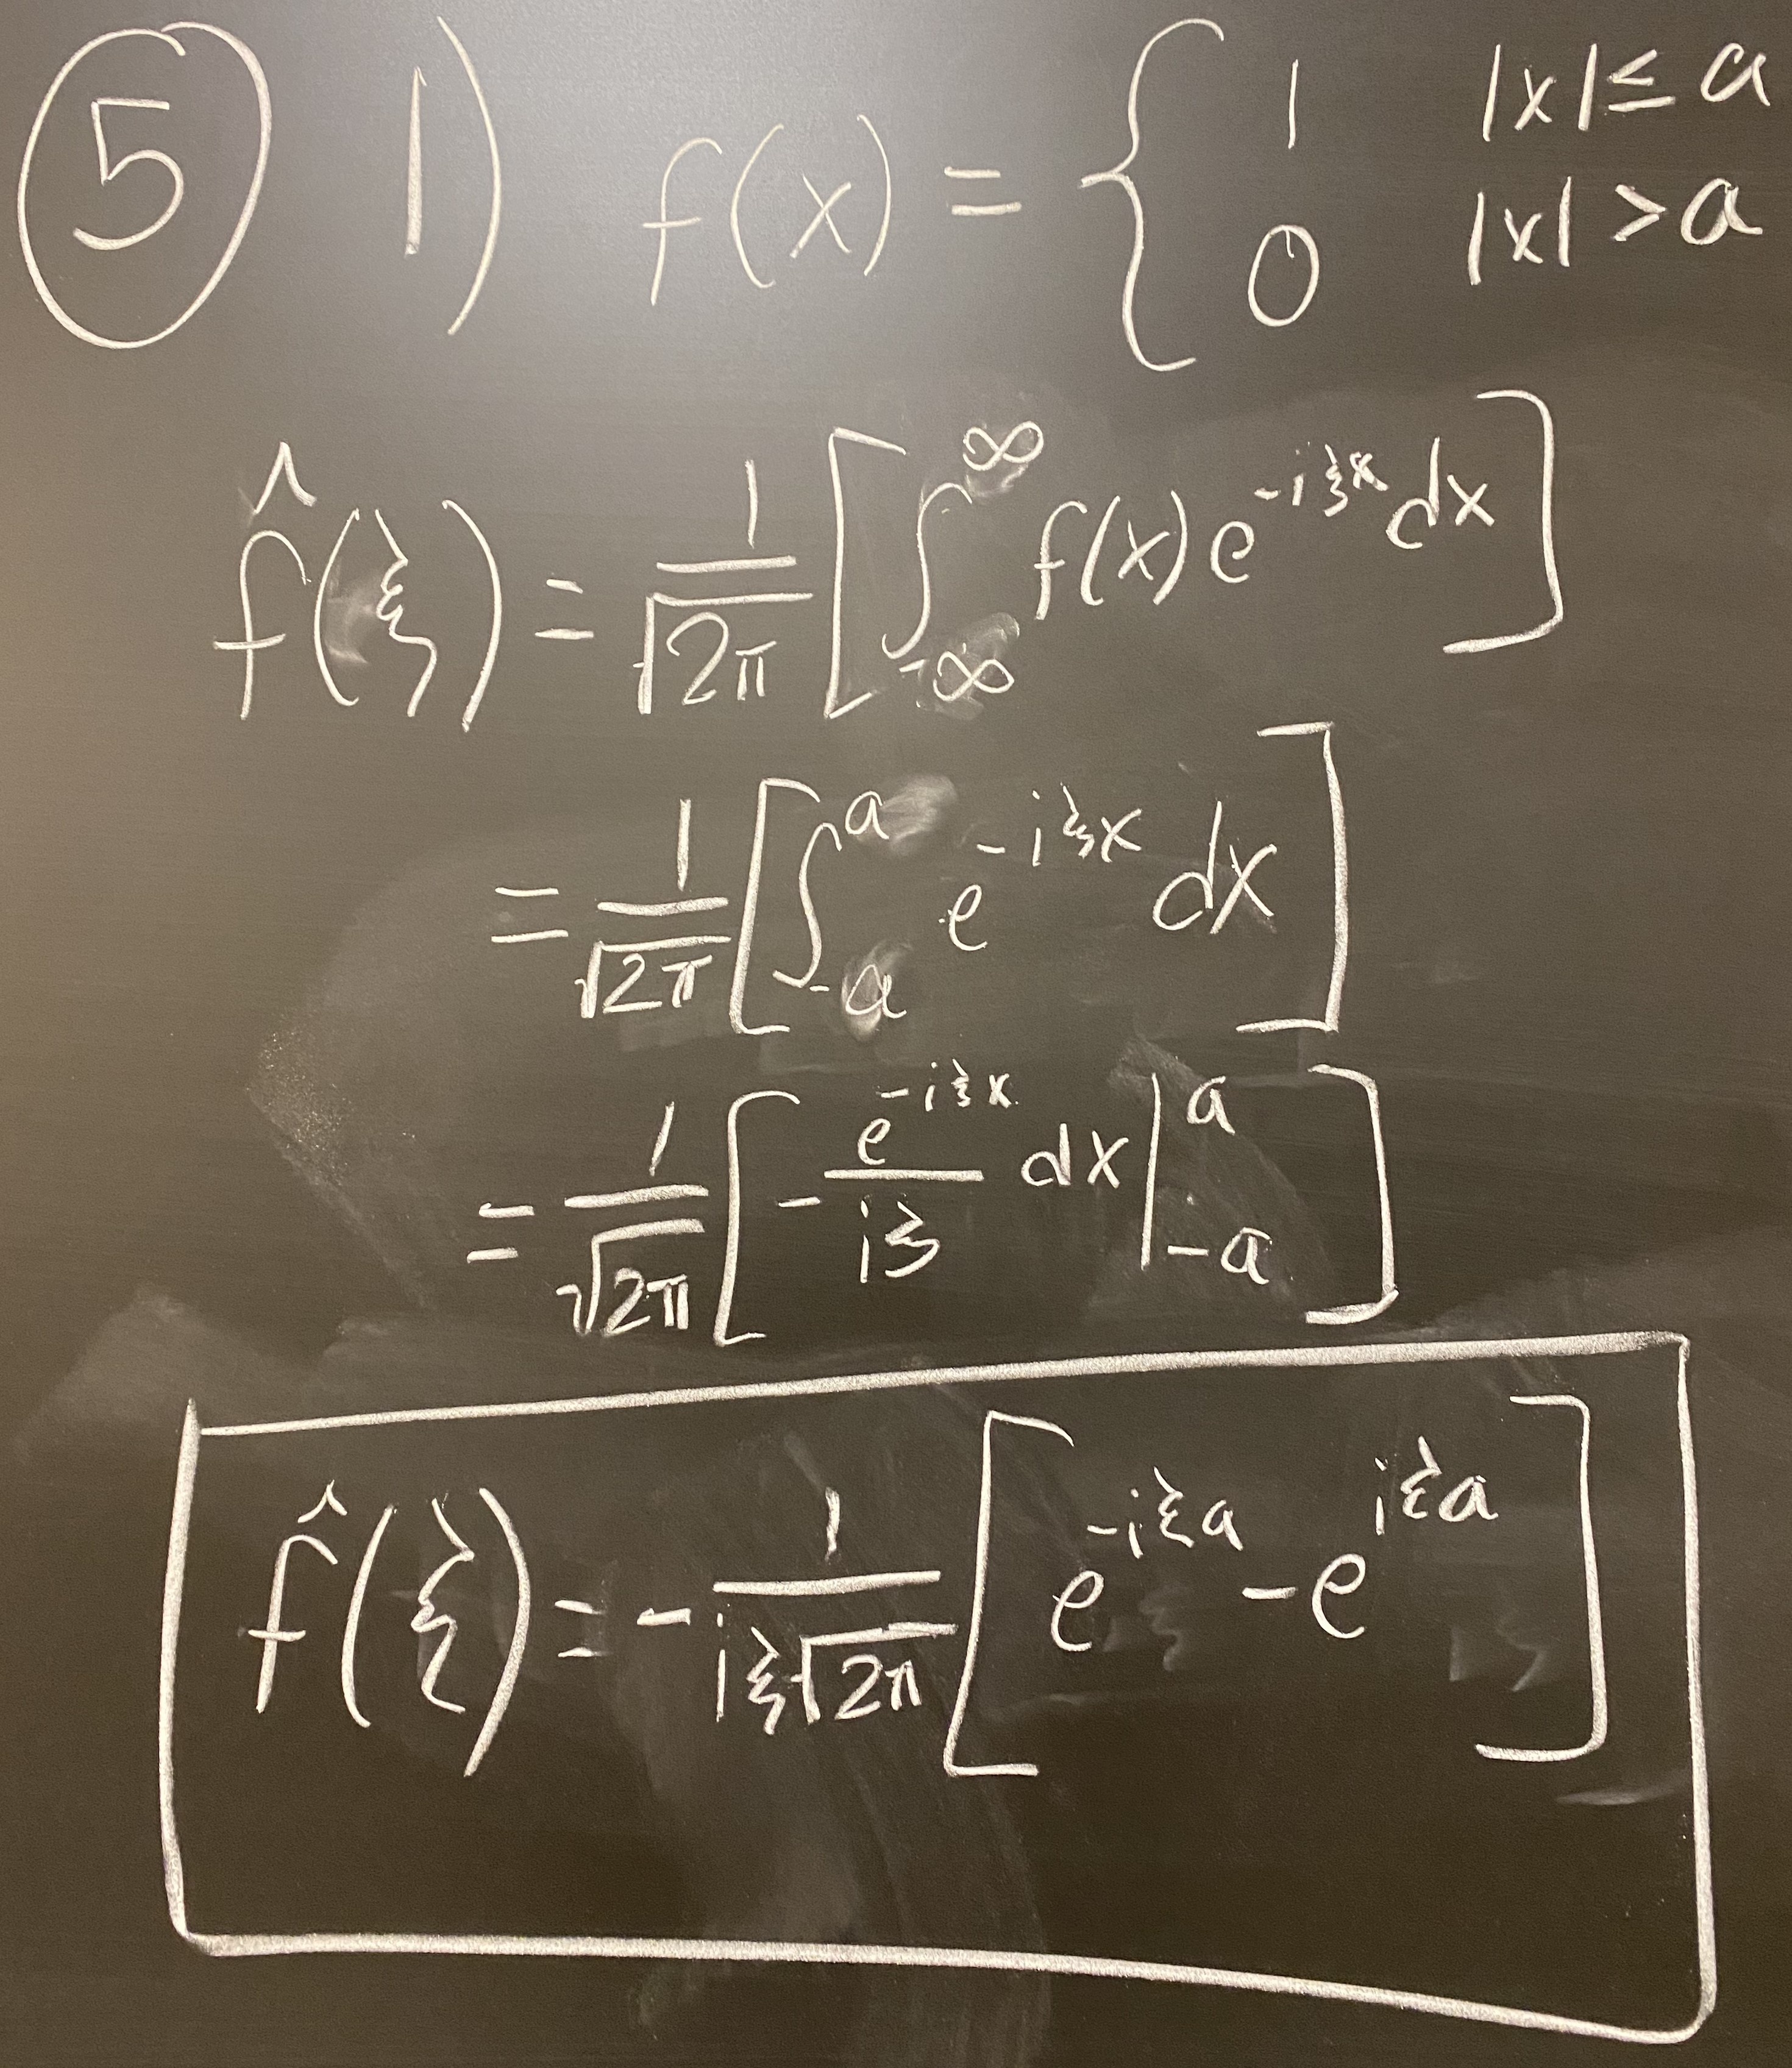
\includegraphics[width = 0.75\textwidth]{Problem 5 Part 1.jpeg}
        \end{figure}

        \item \phantom{.}
        \begin{figure}[H]
            \centering
            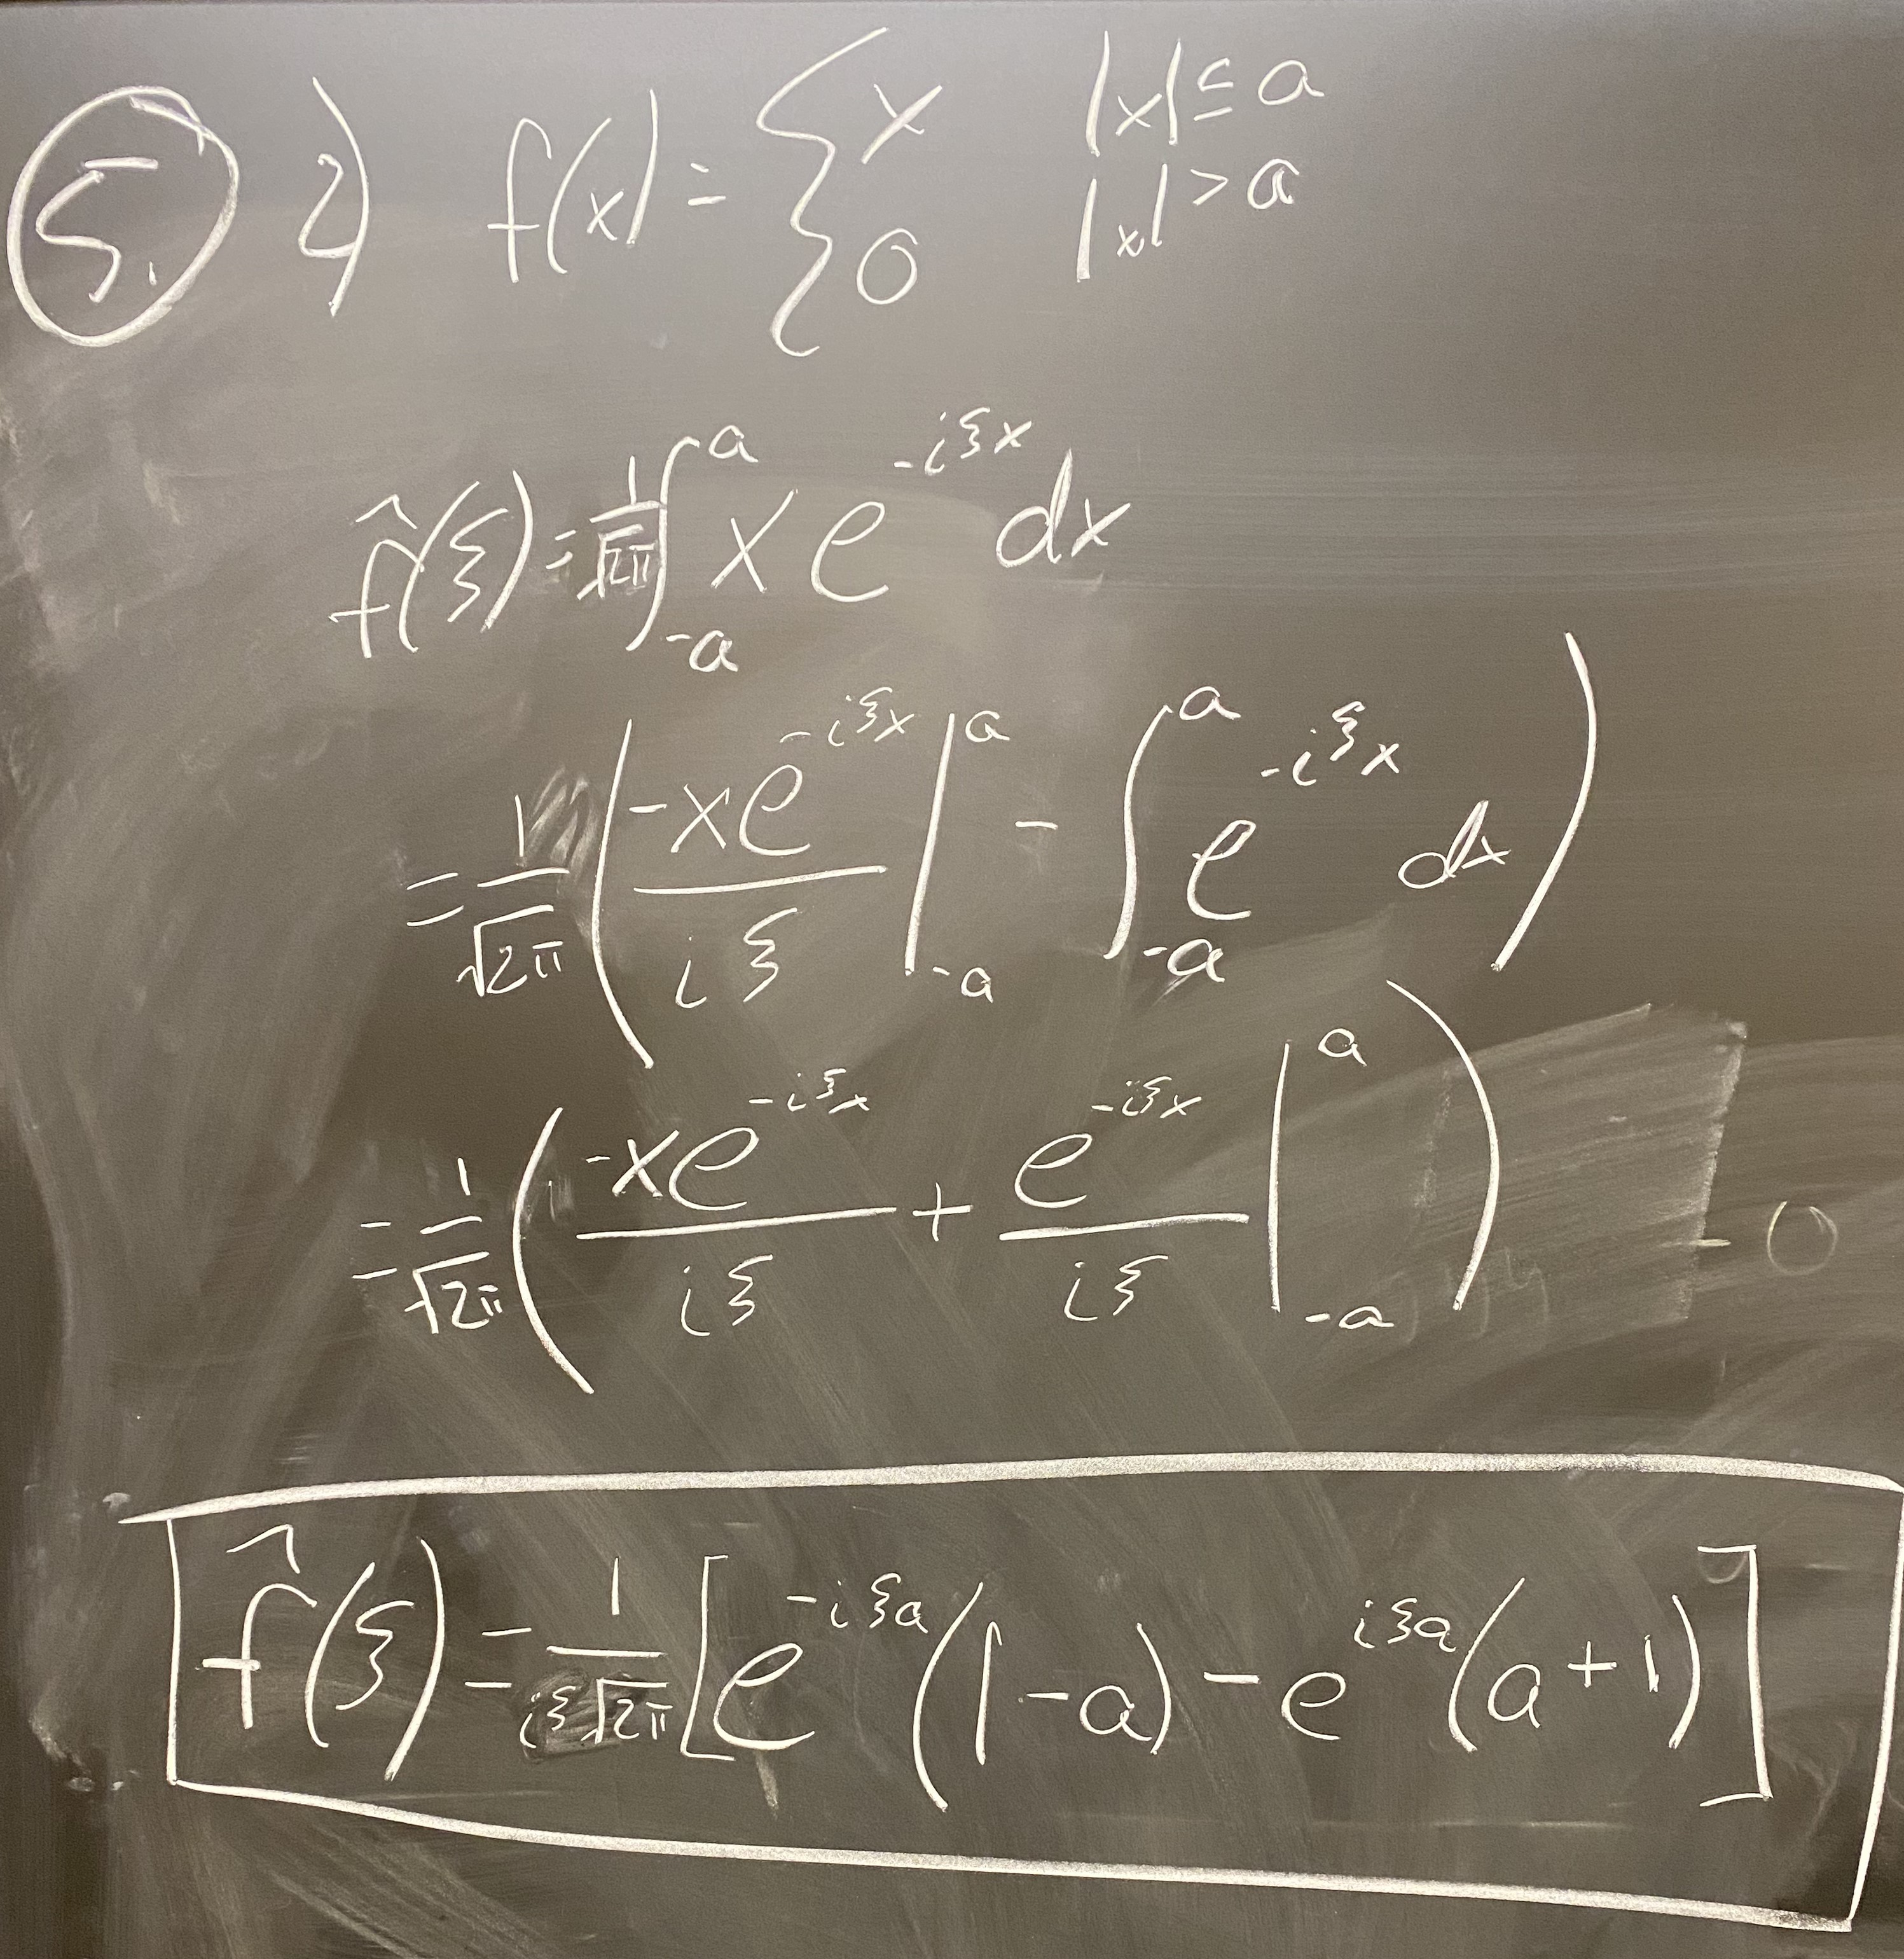
\includegraphics[width = 0.7\textwidth]{Problem 5 Part 2.jpeg}
        \end{figure}

        \item \phantom{.}
        \begin{figure}[H]
            \centering
            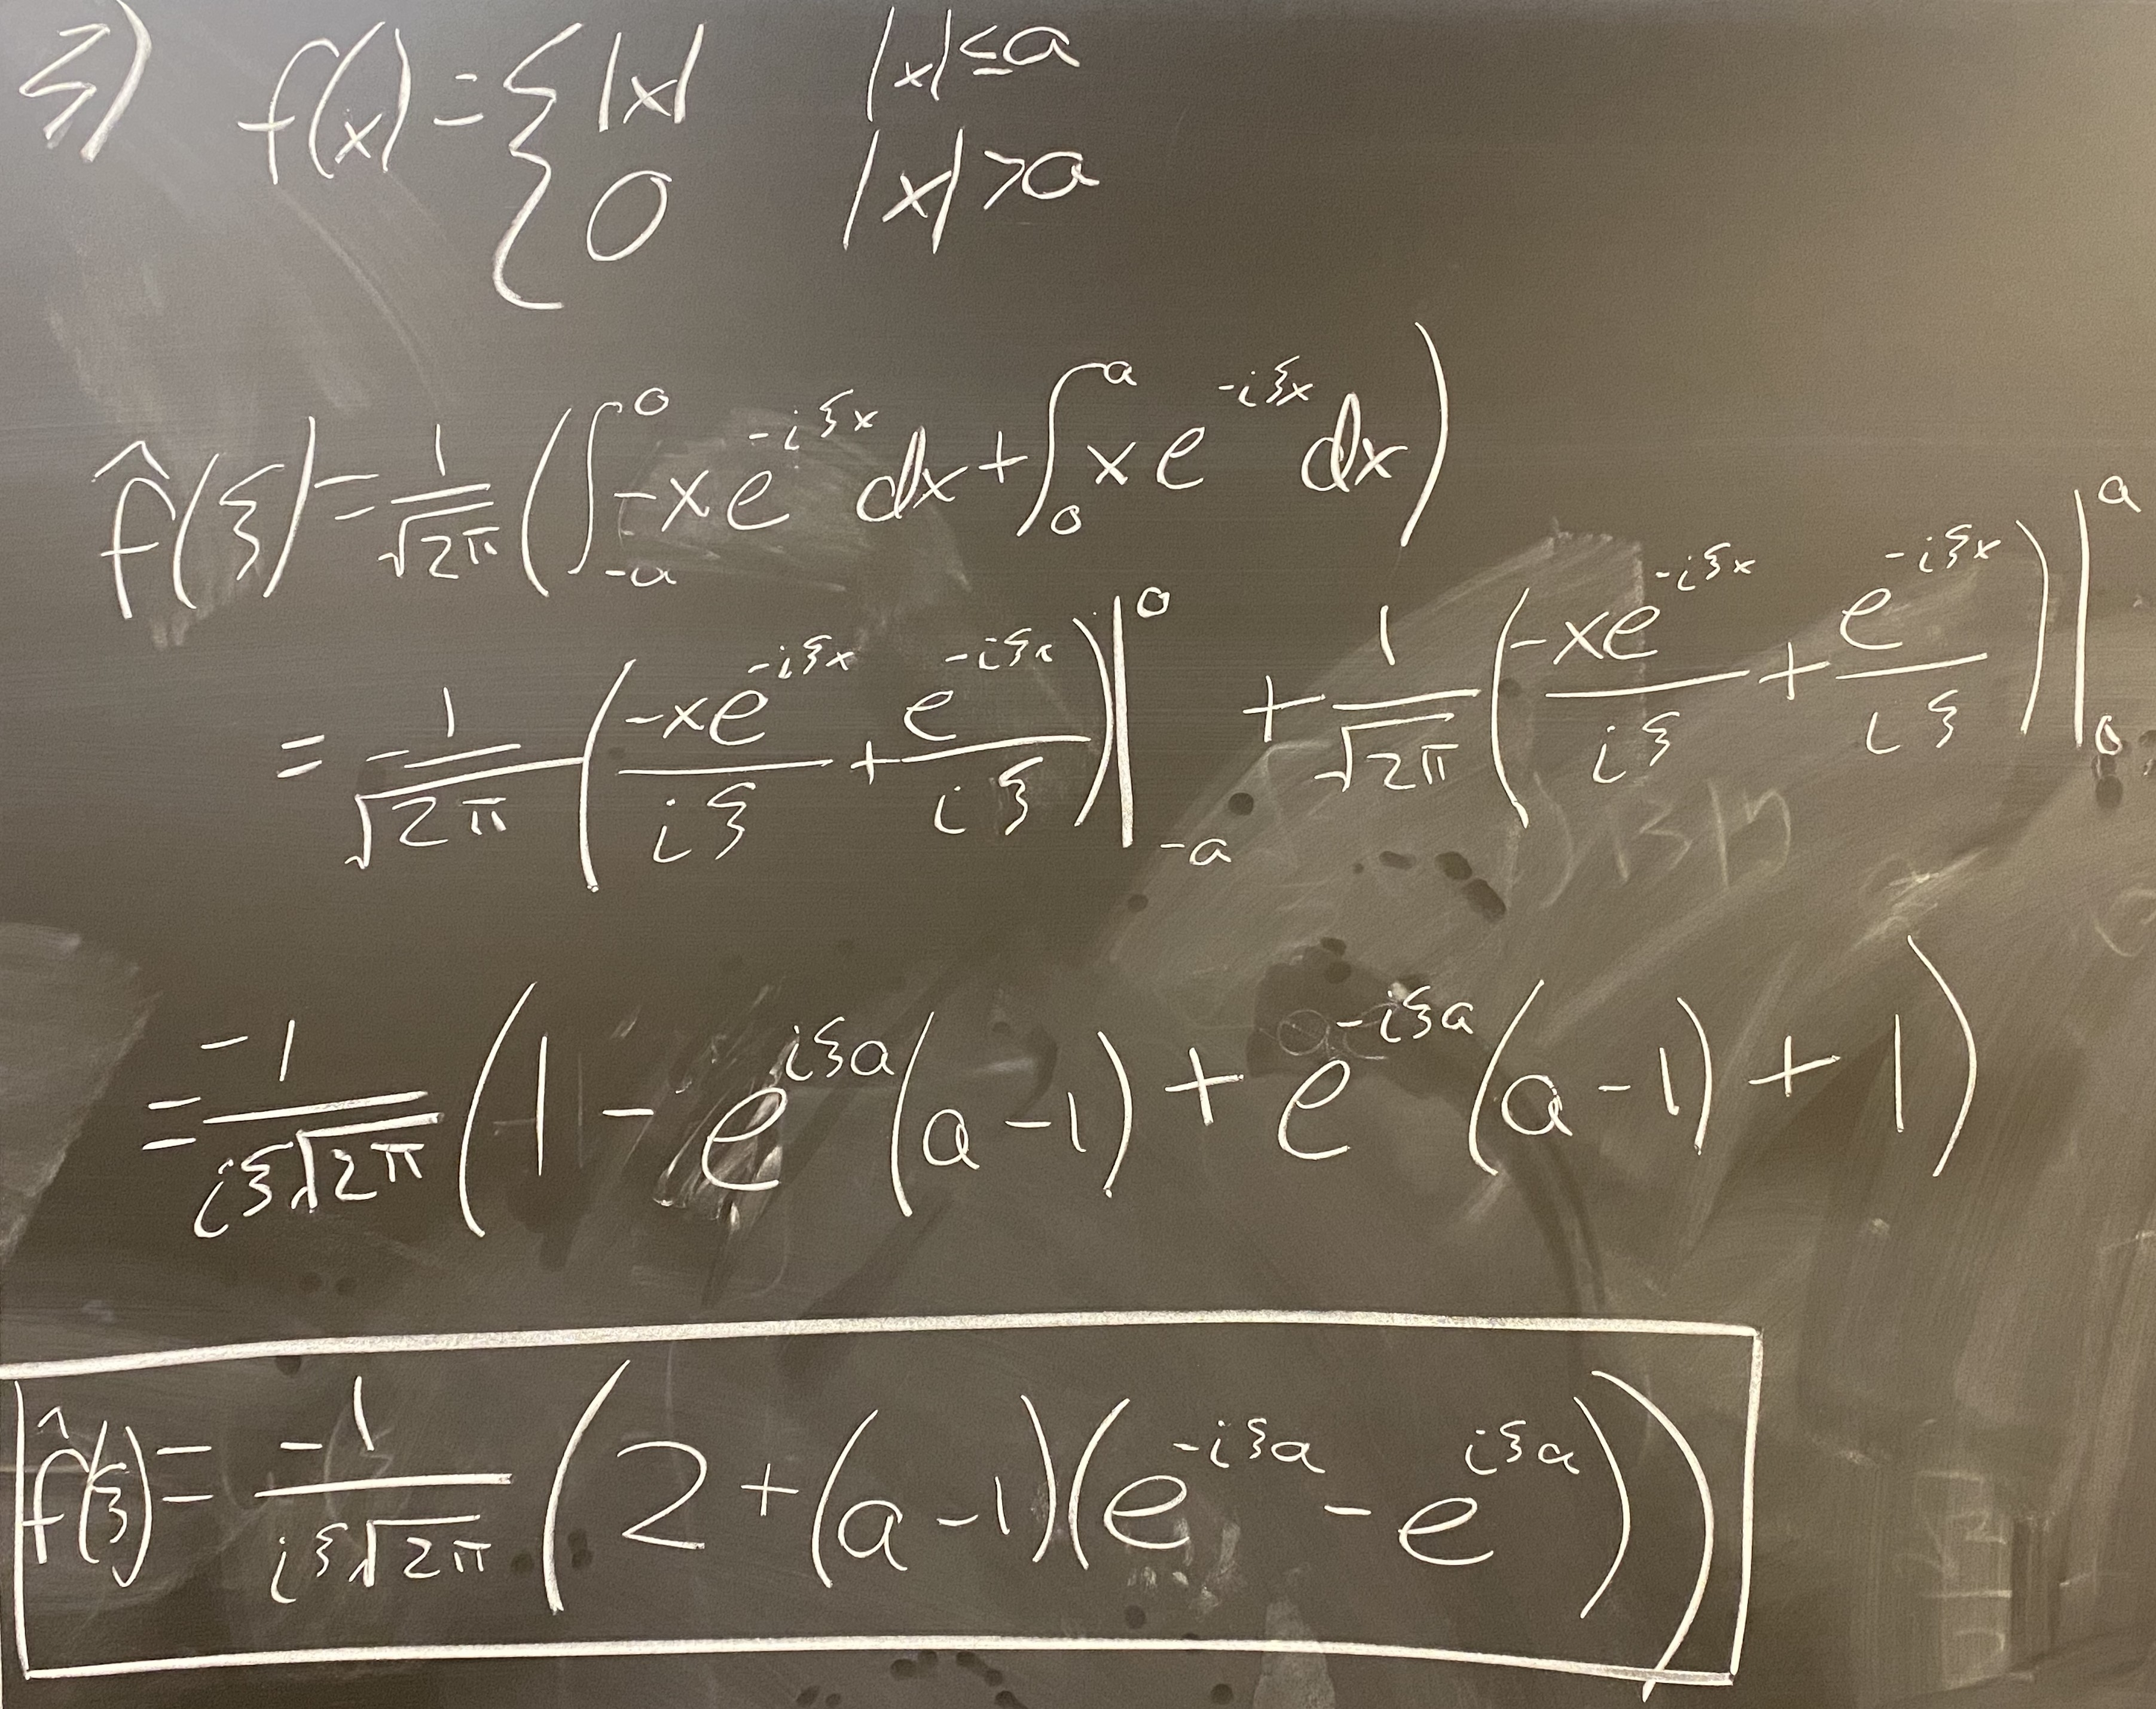
\includegraphics[width = 0.7\textwidth]{Problem 5 Part 3.jpeg}
        \end{figure}

        \item \phantom{.}
        \begin{figure}[H]
            \centering
            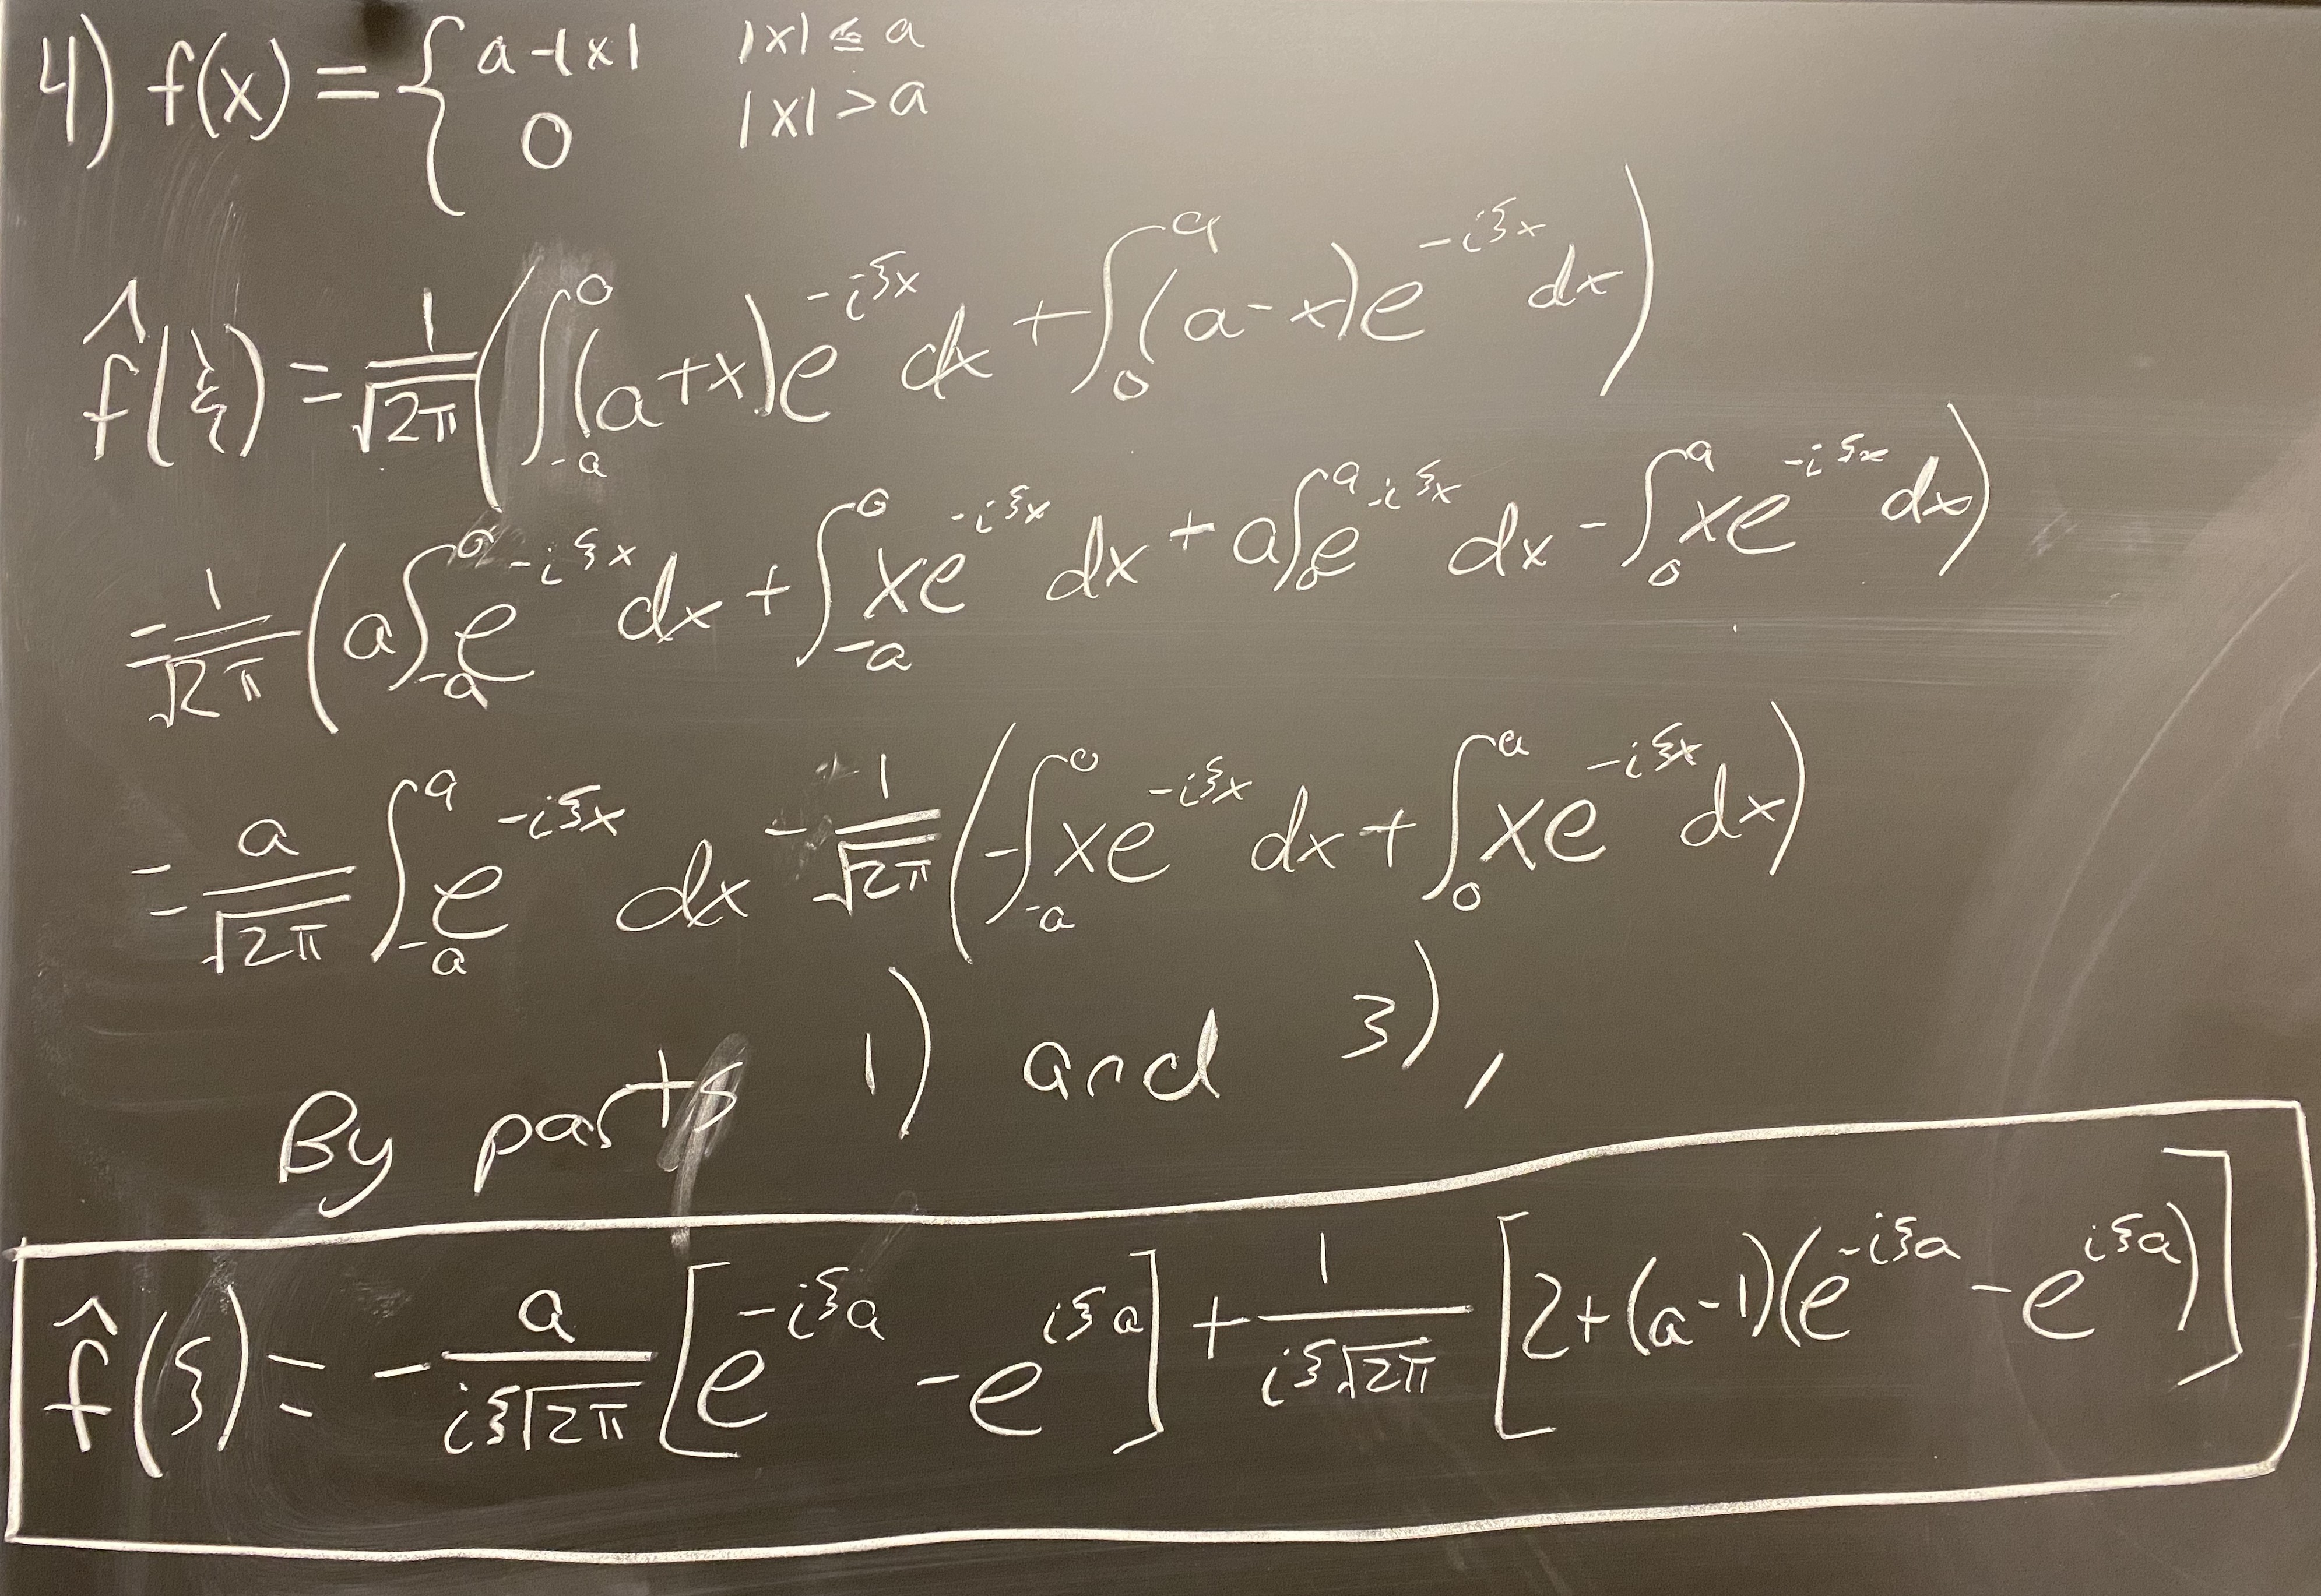
\includegraphics[width = 0.75\textwidth]{Problem 5 Part 4.jpeg}
        \end{figure}

        \item \phantom{.}
        \begin{figure}[H]
            \centering
            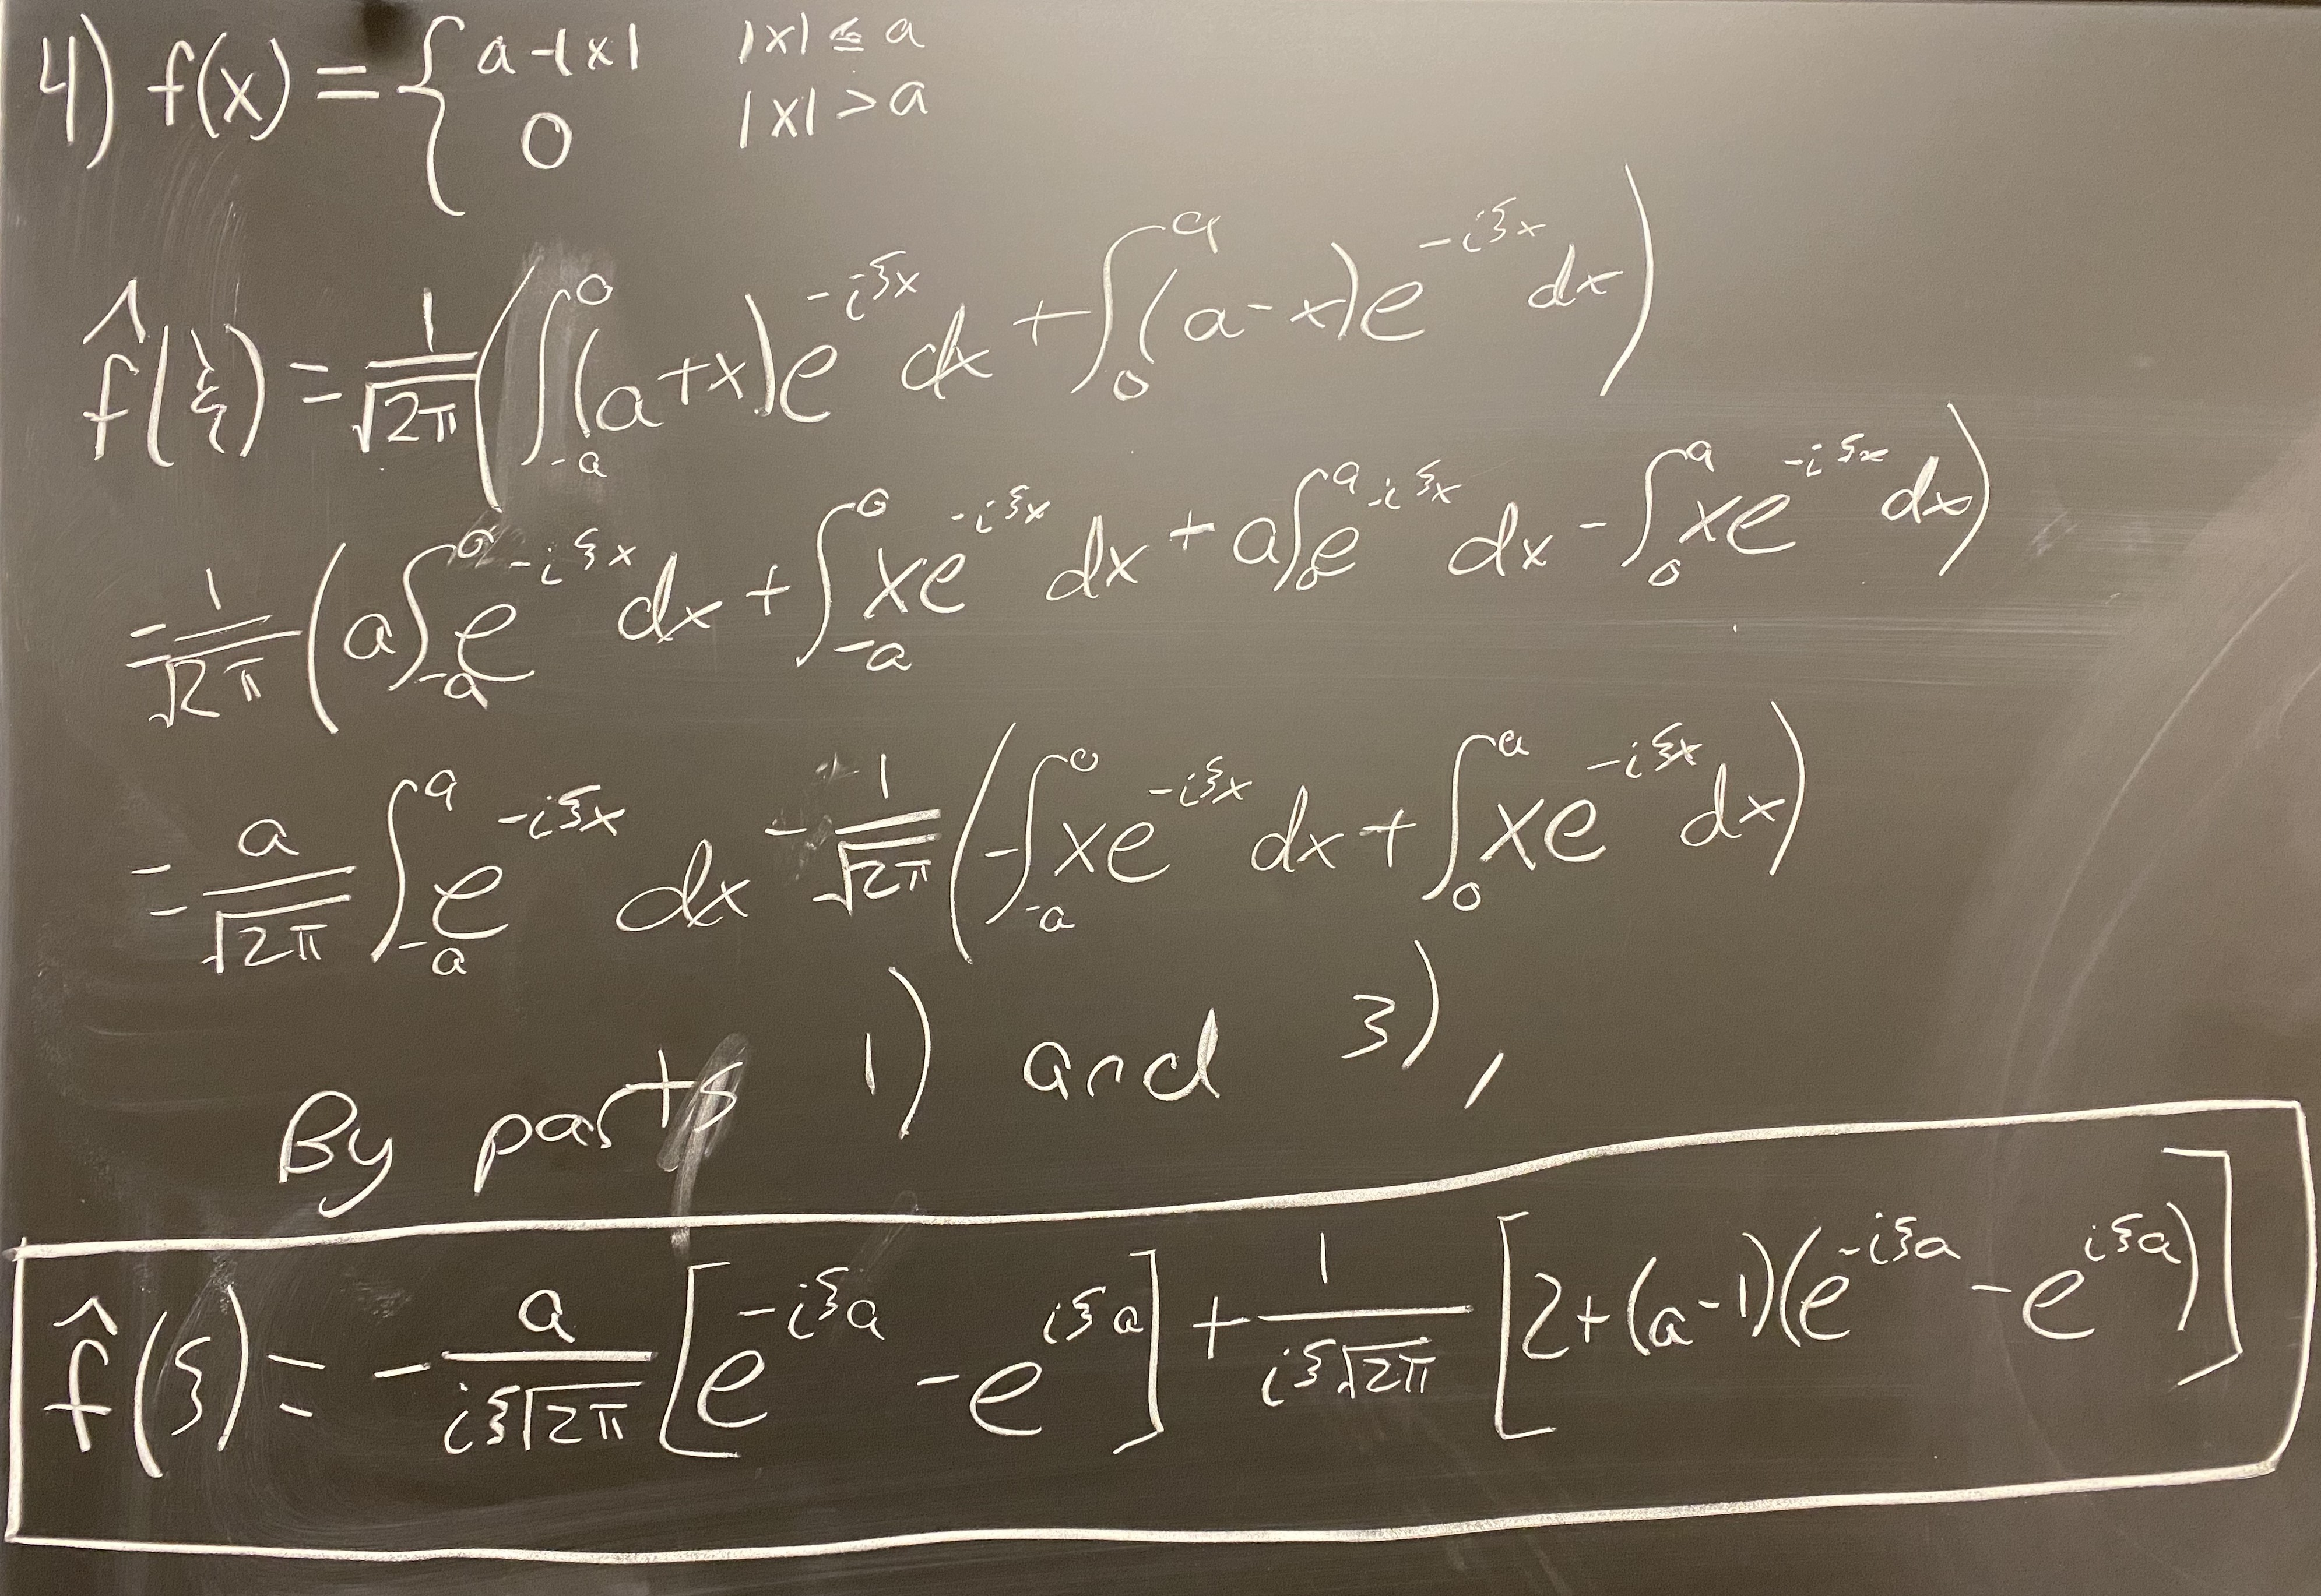
\includegraphics[width = 0.75\textwidth]{Problem 5 Part 4.jpeg}
        \end{figure}

        \item \phantom{.}
        \begin{figure}[H]
            \centering
            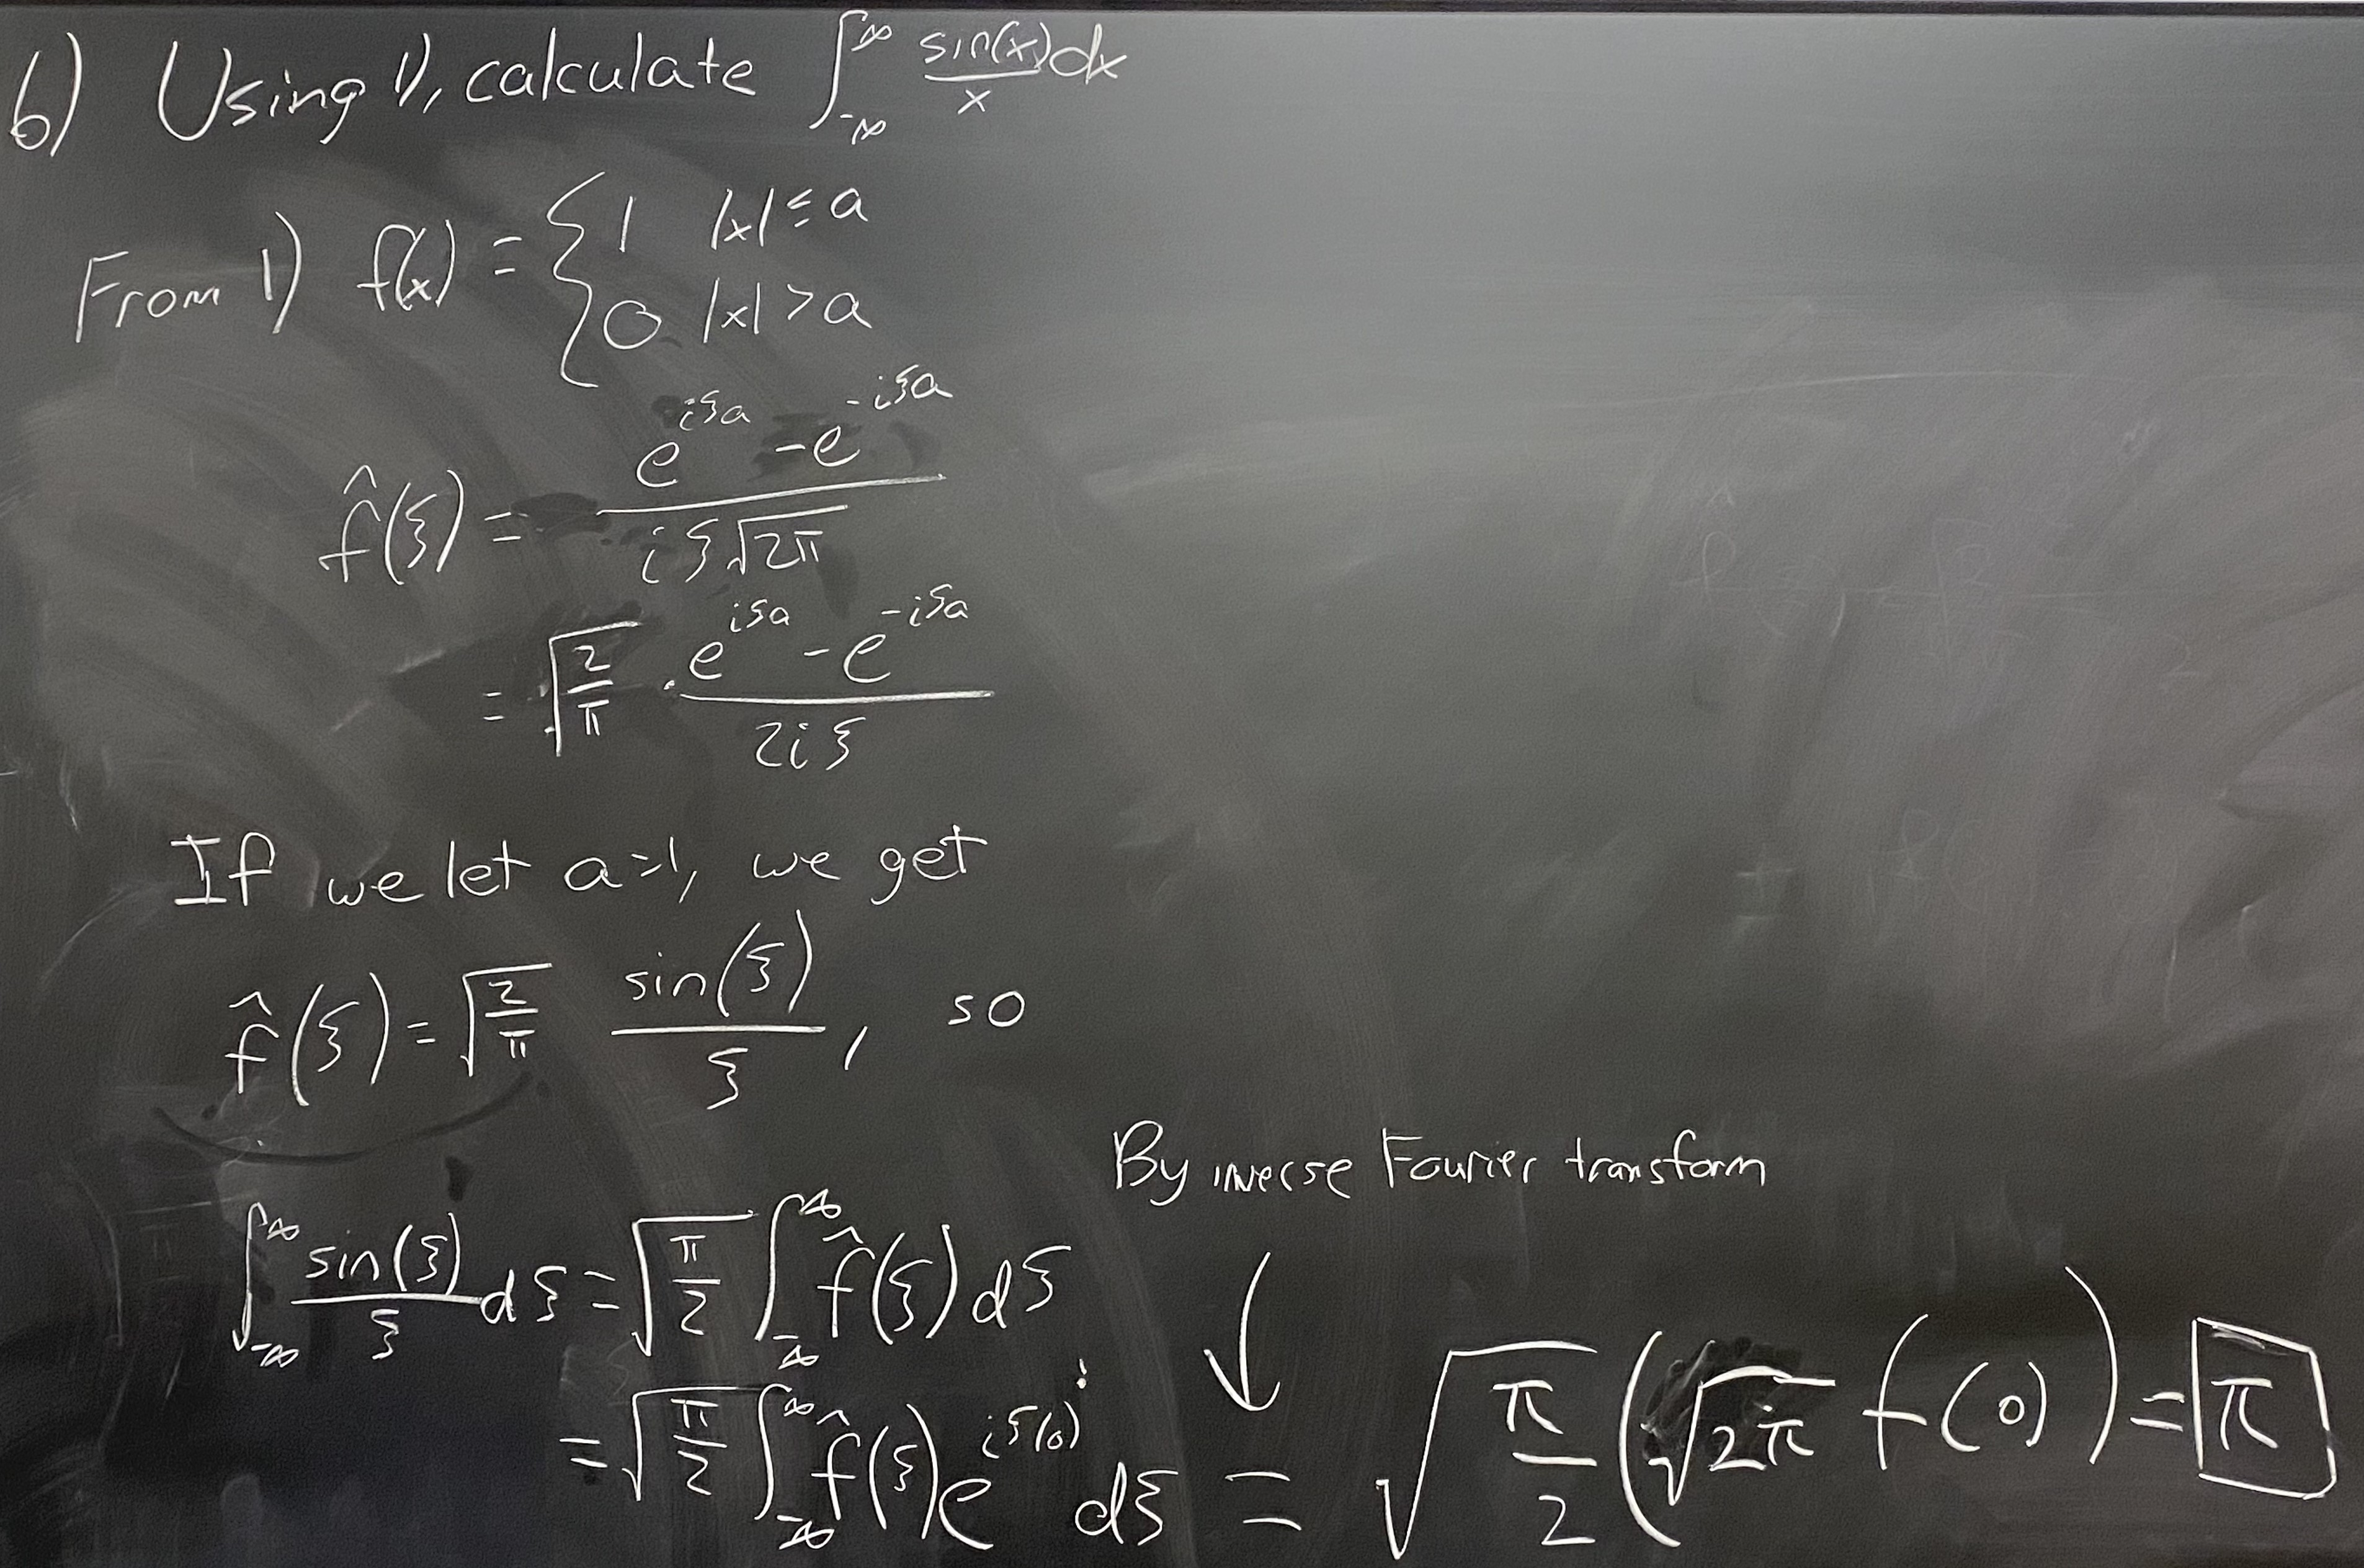
\includegraphics[width = 0.75\textwidth]{Problem 5 Part 6.jpeg}
        \end{figure}
    \end{enumerate}
\end{ans}

\end{document}
